%%%%%%%%%%%%%%%%%%%%%%%%%%%%%%%%%%%%%%%%%%%%%%%%%%%%%%%%%%%%%%%%%%%%%%%%

%%% The code below was generated by the tool at http://dl.acm.org/ccs.cfm.
%%% Please replace this example with code appropriate for your own paper.

%%%%%%%%%%%%%%%%%%%%%%%%%%%%%%%%%%%%%%%%%%%%%%%%%%%%%%%%%%%%%%%%%%%%%%%%

%%% LaTeX Template for AAMAS-2025 (based on sample-sigconf.tex)
%%% Prepared by the AAMAS-2025 Program Chairs based on the version from AAMAS-2025. 

%%%%%%%%%%%%%%%%%%%%%%%%%%%%%%%%%%%%%%%%%%%%%%%%%%%%%%%%%%%%%%%%%%%%%%%%

%%% Start your document with the \documentclass command.


%%% == IMPORTANT ==
%%% Use the first variant below for the final paper (including auithor information).
%%% Use the second variant below to anonymize your submission (no authoir information shown).
%%% For further information on anonymity and double-blind reviewing, 
%%% please consult the call for paper information
%%% https://aamas2025.org/index.php/conference/calls/submission-instructions-main-technical-track/

%%%% For anonymized submission, use this
\documentclass[sigconf,anonymous]{aamas} 
\begin{CCSXML}
<ccs2012>
    <concept>
        <concept_id>10010147.10010178.10010199.10010202</concept_id>
        <concept_desc>Computing methodologies~Multi-agent planning</concept_desc>
        <concept_significance>500</concept_significance>
        </concept>
  </ccs2012>
\end{CCSXML}
\ccsdesc[500]{Computing methodologies~Multi-agent planning}
%%%% For camera-ready, use this
% \documentclass[sigconf]{aamas} 

%%% Load required packages here (note that many are included already).

\usepackage{balance} % for balancing columns on the final page
% new package
\usepackage{algorithm}
% \usepackage{algorithmic}
\usepackage{algpseudocode}
\usepackage{amsmath}
% \usepackage[linesnumbered,ruled,vlined]{algorithm2e}
\usepackage{graphicx}
\usepackage{subfigure}
\usepackage{url}
% \usepackage{epstopdf}
% \usepackage{epsfig}
\renewcommand{\algorithmicrequire}{\textbf{Input:}}
\renewcommand{\algorithmicensure}{\textbf{Output:}}
%%%%%%%%%%%%%%%%%%%%%%%%%%%%%%%%%%%%%%%%%%%%%%%%%%%%%%%%%%%%%%%%%%%%%%%%

%%% AAMAS-2025 copyright block (do not change!)

\setcopyright{ifaamas}
\acmConference[AAMAS '25]{Proc.\@ of the 24th International Conference
on Autonomous Agents and Multiagent Systems (AAMAS 2025)}{May 19 -- 23, 2025}
{Detroit, Michigan, USA}{A.~El~Fallah~Seghrouchni, Y.~Vorobeychik, S.~Das, A.~Nowe (eds.)}
\copyrightyear{2025}
\acmYear{2025}
\acmDOI{}
\acmPrice{}
\acmISBN{}


%%%%%%%%%%%%%%%%%%%%%%%%%%%%%%%%%%%%%%%%%%%%%%%%%%%%%%%%%%%%%%%%%%%%%%%%

%%% == IMPORTANT ==
%%% Use this command to specify your EasyChair submission number.
%%% In anonymous mode, it will be printed on the first page.

\acmSubmissionID{<<EasyChair submission id>>}

%%% Use this command to specify the title of your paper.

\title[AAMAS-2025 Formatting Instructions]{Task Group Allocation for Solving Multi-Load Agent Pickup and Delivery problem}

%%% Provide names, affiliations, and email addresses for all authors.

\author{Hao Ye}
\affiliation{
  \institution{Harbin Institute of Technology (Shenzhen)}
  \city{Shenzhen}
  \country{China}}
\email{yehao@stu.hit.edu.cn}

\author{Yifei Li}
\affiliation{
  \institution{Harbin Institute of Technology (Shenzhen)}
  \city{Shenzhen}
  \country{China}}
\email{liyifei@stu.hit.edu.cn}

% \author{Hejiao Huang}
% \affiliation{
%   \institution{Harbin Institute of Technology (Shenzhen)}
%   \city{Shenzhen}
%   \country{China}}
% \email{huanghejiao@hit.edu.cn}

%%% Use this environment to specify a short abstract for your paper.

% \begin{abstract}
% This paper addresses the multi-load agent pickup and delivery problem (MLAPD),
% in which a set of agents needs to efficiently complete a set of dynamically arriving tasks.
% Sepcially, in MLAPD, each agent can carry multiple tasks simultaneously.
% Therefore, tasks, which are executed by the same agent simultaneously,
% affect each other's completion time.
% This is difficult to schedule task groups with low effect on each other to agents.
% To address this issue, we propose a Task Group Allocation (TGA) algorithm 
% to minimum the completion time of all tasks.
% We first quantify the carpooling chance between multiple tasks,
% and then divide the set of tasks into groups via 
% K-Capacity Hierarchical Clustering Algorithm.
% Finally, we allocate task groups to agents.
% Experimental results show that the TGA algorithm outperforms 
% the state-of-the-art algorithms in terms of service time, makespan, and processing time.
% \end{abstract}

\begin{abstract}
  This paper addresses the multi-load agent pickup and delivery problem (MLAPD),
  in which the multi-load agent set is required
  to efficiently complete a set of dynamically arriving tasks.
  Note that each multi-load agent can carry multiple tasks simultaneously,
  which causes that multiple tasks may affect each other's completion time.
  Therefore, it is difficult to assign multiple tasks to the most suitable agents
  and schedule the completion order of them.
  To address this issue, we propose a Task Group Allocation algorithm (TGA)
  to minimum the completion time of all tasks.
  We first quantify the carpooling scores between multiple tasks,
  and then divide the set of tasks into groups,
  in which tasks in the same group have little influence on each other,
  via proposed K-Capacity Hierarchical Clustering Algorithm (KCHC).
  Finally, we allocate task groups to agents.
  Experimental results show that the TGA algorithm outperforms 
  the state-of-the-art algorithms in terms of service time, makespan, and processing time.
\end{abstract}

%%% The code below was generated by the tool at http://dl.acm.org/ccs.cfm.
%%% Please replace this example with code appropriate for your own paper.


%%% Use this command to specify a few keywords describing your work.
%%% Keywords should be separated by commas.

\keywords{Multi-load agent, Pickup and delivery problem, Task allocation}

%%%%%%%%%%%%%%%%%%%%%%%%%%%%%%%%%%%%%%%%%%%%%%%%%%%%%%%%%%%%%%%%%%%%%%%%

%%% Include any author-defined commands here.


         
\newcommand{\BibTeX}{\rm B\kern-.05em{\sc i\kern-.025em b}\kern-.08em\TeX}

%%%%%%%%%%%%%%%%%%%%%%%%%%%%%%%%%%%%%%%%%%%%%%%%%%%%%%%%%%%%%%%%%%%%%%%%

\begin{document}

%%% The following commands remove the headers in your paper. For final 
%%% papers, these will be inserted during the pagination process.

\pagestyle{fancy}
\fancyhead{}

%%% The next command prints the information defined in the preamble.

\maketitle 

\section{Introduction}
\label{sec:introduction}
Recently, the multi-agent pickup and delivery (MAPD) problem has attracted increasing attention,
because it can be applied to various fields, 
such as warehouse robots for handling goods,
aircraft towing robots for aircraft movement,
and office delivery robots~\cite{li2021lifelong, ma2019lifelong, wurman2008coordinating}.
In the MAPD problem, a set of agents need to complete a set of dynamically arriving tasks.
When a task is released, the system needs to allocate it to an agent.
Then, the agent needs to arrive at the pickup location to pick task up 
and delivery task to the delivery location.
Note that the agent is single-load and can only carry one task once time, in the MAPD problem.
Now, many platforms have used multi-load agents to complete tasks.
Multi-load agents can carry multiple tasks simultaneously
to adapt to the complex environment and improve the efficiency of the system~\cite{shi2022adaptive, chen2021integrated}.

Existing works focusing on the task allocation of MLAPD problem can be divided into two main types.
Fisrt, some works~\cite{wu2021multi,zhang2022effective,wang2024task} focus on individual task assignments.
These works find the connection between individual tasks and agents,
and then use a special strategy for task allocation.
However, matching between individual tasks and agents can lead the problem to a local optimum easily.
Second, some works~\cite{bai2022group,electronics12183842} focus on the task group assignments,
which divide the set of tasks into groups,
Then allocate task groups to agents.
However, these works have excessive computational time and no theoretical support.

There exits a main challenge in the MLAPD problem.
When a agent is carrying multiple tasks
and going to the pickup location or delivery location of a task,
it maybe make a detour to pick up or deliver another task.
So, tasks,
which are allocated to the same agent simultaneously,
affect each other's completion time.
A unreasonable allocation of tasks to agents will 
lead to a longer completion time of all tasks.
Therefore, it is difficult to assign multiple tasks to the most suitable agents 
and schedule the completion order of them,
to minimum the completion time of all tasks.

To address this issue,
we analyze the likelihood of carpooling between two task.
Then, we evaluate the upper bound on the cost of the schedule of multiple tasks,
and proof it.
Based on it, we quantify the carpooling scores between multiple tasks,
and propose the K-Capacity Hierarchical Clustering Algorithm (KCHC).
KCHC algorithm divides the set of tasks into groups,
where tasks in the same group have little influence on each other.
Finally, we introduce the Task Group Allocation Algorithm (TGA) to allocate task groups to agents.
Experimental results show that the TGA algorithm outperforms,
compared to the state-of-the-art algorithms
in terms of service time, makespan, and processing time.
% we propose a Task Group Allocation algorithm (TGA)
% to minimum the completion time of all tasks.
% TGA algorithm divides the set of tasks into groups,
% where tasks in the same group have little influence on each other,
% and then allocate task groups to agents.
% In the beginning, we analyze the likelihood of carpooling between each task.
% Then, we quantify the carpooling scores between multiple tasks,
% and proof its validity.
% Based on this, we present K-Capacity Hierarchical Clustering Algorithm (KCHC)
% to divide the set of tasks into groups,
% where tasks in the same group have little influence on each other.
% Finally, we introduce the Task Group Allocation Algorithm 
% to allocate task groups to agents.
% Experimental results show that the TGA algorithm outperforms,
% compared to the state-of-the-art algorithms
% in terms of service time, makespan, and processing time.

The rest of this paper is organized as follows.
In Section~\ref{sec:related}, we review the related work on the pickup and delivery problem.
Section~\ref{sec:problem} presents the definition of MLAPD problem.
In Section~\ref{sec:solution}, we introduce the Task Group Allocation Algorithm to solve the MLAPD problem.
We show the experimental results in Section~\ref{sec:experiment}
and conclude the paper in Section~\ref{sec:conclusion}. 

\section{Related Work}
\label{sec:related}
This section reviews the related works on the multi-agent pickup and delivery problem (MAPD) 
and the multi-load agent pickup and delivery problem (MLAPD).
\subsection{MAPD problem}
\label{sec:SLAPD}
In MAPD problem, each agent can only carry one task once time.
The MAPD problem has been widely studied in the existing works~\cite{ma2017lifelong,wu2021multi,zhou2019balanced,wang2023efficient}.

To solve this problem, 
Ma et al.~\cite{ma2017lifelong} present Token Passing (TP) 
and Token Passing with Task Swaps (TPTS). 
TP plans its paths for the agents in turn, 
and its task set contains all tasks that are not assigned to agents. 
Compared with TP, the task set of TPTS contains all unfinished tasks.
For maximizing the completion ratio of tasks,
Wu et al.~\cite{wu2021multi} take an integrated approach,
which allocates and plans a task at a time.
They define the priority of tasks based on the release time and the deadline,
and propose a prioritization-based framework for combined task assignment and path planning.
Moreover, they utilize the boundary and pruning techniques
in the proposed framework to greatly improve the computational efficiency.
Howerver, single-load agents cannot satisfy all the requirements of reality,
since load capacity limitations.
Different from other work,
Zhou et al.~\cite{zhou2019balanced} focus on the min-max balanced connected q-partition problem
that seeks the early completion time of a multi-agent system while satisfying task constraints.
This study presents the first exact Mixed Integer Linear Programming (MILP) in the literature,
which can partition any graph into a given number of arbitrary components,
and a genetic algorithm to solve the BCPq problem.
In~\cite{wang2023efficient}, 
an effective and efficient performance impact (EEPI) algorithm 
is proposed based on the performance impact (PI) algorithm. 
First, the travel time from each vehicle's initial position to its task position is minimized,
allowing more time to be left for the vehicle to perform more tasks due to limited fuel.
Second, the start time of each task should be close enough to its deadline 
so that tasks with earlier deadlines can be assigned earlier than tasks with later deadlines.
Howerver, these works focus on the single-load agent pickup and delivery problem,
which cannot apply all the real-world scenarios.
Therefore, we present our approach to solve the MLAPD problem efficiently.

\subsection{MLAPD problem}
\label{sec:MLAPD}
In MLAPD problem, each agent can carry multiple tasks simultaneously.
Therefore, MLAPD problem is more complex than MAPD,
but it has more practical significance in real-world applications.

Sarkar et al.~\cite{sarkar2018scalable} proposed a heuristic algorithm
nearest-neighbor based Clustering and Routing (nCAR) to solve the MLAPD problem.
nCAR algorithm first clusters tasks based on the nearest neighbor,
and then constructs a route for each cluster by mapping it to a traveling salesman problem.
Zhang et al.~\cite{zhang2022effective} considering 
introduce an improved iterated greedy (IIG) algorithm.
IIG algorithm first generates an initial solution by a greedy strategy,
and then iteratively improves the solution by a local search strategy.
Sepcially, IIG algorithm designs two rules to fast identify unfeasible solutions.
In~\cite{bai2022group}, two group-based distributed auction algorithms are designed
to solve this task allocation problem. 
Guided by the auction algorithms,
the agents first distributedly compute the feasible parcel groups they can serve,
and then communicate to find parcel group assignments. 
Howerver, group-based distributed auction algorithms calculate all possible parcel groups,
which is time-consuming.
To cope with uncertain scenarios,
Wilde et al.~\cite{wilde2024statistically} present an adaptive sampling algorithm
that finds MAPD solutions that approximate the expected Pareto front
and ensure that the solutions are statistically distinguishable.
Wang et al.~\cite{wang2024task} define a novel recurrent open shop scheduling (ROSS) problem
variant with unique sequence structure.
New sequence and scheduling models are extended to accommodate it.
Then, problem-specific additive beam Christofides (ABC) construction heuristics,
greedy local search (GLS) and simulated annealing (SA) meta-heuristics 
are designed accordingly.
You et al.~\cite{electronics12183842} transform the MLAPD problem into
a multi-traveler salesman problem (MTSP) with time windows,
using a multi-angle K-means clustering algorithm.
Then, they propose a two-stage load-balancing strategy,
in which the first stage is making a large adjustment to unbalanced task set,
and the second stage is making a small adjustment to the balanced task set.
While these works have made significant progress in the MLAPD problem,
they do not consider the impact of tasks on each other's completion time.
Therefore, we present our approach to solve the MLAPD problem efficiently.

\section{PROBLEM DEFINITION}
\label{sec:problem}
In this section, we introduce the multi-load agent pickup and delivery problem, 
which we address in this paper. 
Before this, we first give the definitions of map, task, agent, comparative metrics, and MLAPD problem.

\begin{definition}[Map]
\label{MapDfn}
    A map $G = (V, E)$ is the, 
    whose vertices set $V$ correspond to locations and edges set $E$ represent routes between adjoining locations.
    The shortest distance of the path between two locations $v_{i}$ and $v_{j}$ is denoted as $dis(v_{i}, v_{j})$.

\end{definition}

\begin{definition}[Task]
\label{TaskDfn}
    A task $\tau \in \Gamma$ is a tuple 
    $<v^{s}_{\tau}, v^{g}_{\tau}, t^{r}_{\tau}, t^{c}_{\tau}>$, 
    where $v^{s}_{\tau}$ and $v^{g}_{\tau}$ are the pickup location and delivery location, respectively. 
    $t^{r}_{\tau}$ and $t^{c}_{\tau}$ are the release and completed time, respectively.
\end{definition}

% Task Group ?

\begin{definition}[Agent]
\label{AgentDfn}
    An agent $a \in A$ is represented as a tuple $<v_{a}, c_{a}, \Gamma_{a}, S_{\Gamma_{a}}>$, 
    where $v_{a}$ is location, $c_{a}$ represents the maximum capacity, 
    $\Gamma_{a}$ is the set of tasks, and $S_{\Gamma_{a}}$ is the schedule of $\Gamma_{a}$. 
    The $S_{\Gamma_{a}} = <v_{1}, v_{2},..., v_{n}>$, 
    where $v_{i}$ is a pickup or delivery location of task $\tau \in \Gamma_{a}$,
    and the cost of schedule $S_{\Gamma_{a}}$ is denoted as 
    $Cost(S_{\Gamma_{a}}) = \sum^{n-1}_{i=1}{dis(v_i, v_{i+1})}$.
\end{definition}

A task $\tau \in \Gamma$ is released at $t^{r}_{\tau}$. 
When system assigns $\tau$ to an agent $a$, 
$a$ needs to reach $v^{s}_{\tau}$, 
and then deliver $\tau$ to $v^g_{\tau}$ while recording the completed time $t^{c}_{\tau}$. 


\begin{definition}[Comparative metrics]
    In this paper, we demonstrate algorithmic superiority through three comparative metrics, 
    service time (${ST}$), makespan ($MS$) and processing time ($PT$). 
    $ST = \sum_{\tau_i \in \Gamma}{(t^{c}_{\tau_i} - t^{r}_{\tau_i})}$, 
    is defined as the sum of differences between the completed times and the release times of all tasks.
    $MS = max{\{t^{c}_{\tau}\}}$ $(\forall \tau \in \Gamma)$ 
    is time when last task has completed.
    % $CR = {\sum_{\tau_i \in \Gamma}{X_{\tau_i}}}/{|\Gamma|}$, 
    % where $X_{\tau_i}$ is a decision variable, is completion ratio of $\Gamma$.
    % If task $\tau_{i}$ is completed, then $X_{\tau_i}$ is 1; otherwise, it is 0.
    $PT$ is the average processing time within each batch.
       
\end{definition}

\begin{definition}[MLAPD]
\label{ProDfn}
    Given a map $G$, a set of agents $A$, and a set of tasks $\Gamma$,
    in each batch, the goal of
    the multi-load agent pickup and delivery problem (MLAPD) is to find the allocation of tasks to agents,
    which optimize three comparative indicators, ($ST, MS, PT$).
    Time is discretized into timesteps, and agents can only move to adjacent locations
    or wait at its current location in one timestep.
    To focus on the task allocation, we ignore the time required to avoid conflicts.
    % The multi-load agent pickup and delivery problem (MLAPD) is a tuple $P = <G, A, \Gamma>$, 
    % defined by a map $G$, a set of agents $A$, and a set of tasks $\Gamma$. 
    % Moreover, $P$ amounts to finding the allocation of tasks to agents, 
    % which optimize three comparative indicators, ($ST, MS, PT$).
    % Time is discretized into timesteps, and agents can only move to adjacent locations 
    % or wait at its current location in one timestep.
    % To focus on the task allocation, we ingore the time required to avoid conflicts.
    % Howerver, a conflict occurs when two agents are at the same location or pass through the same edge simultaneously.
    % The time required to avoid conflicts needs to be considered, since it will affect the comparative metrics.
    % Therefore, we assue that agents can take $\theta$ time to avoid a conflict.
\end{definition}
 
\section{Solution}
\label{sec:solution}
In this study, Task-Group Allocation Algorithm is developed to solve MLAPD problem efficiently. 
The TGA method first analyzes the likelihood of carpooling between each task, 
and then quantifies the carpooling scores between multiple tasks to evaluate the impact of tasks on each other's completion time.
Based on this, we present K-Capacity Hierarchical Clustering Algorithm (KCHC) to divide the set of tasks into groups,
where tasks in the same group have little influence on each other.
Finally, we introduce the Task Group Allocation Algorithm to allocate task groups to agents.

\subsection{Carpooling Scores}
% 说明为什么搞task group
The biggest difference between multi-load agent and single-load agent 
is that multi-load agent can load multiple tasks simultaneously. 
This means that multi-load agent performing a task affects the completion time of the "co-passenger" tasks 
which are also executed to the same agent at same time.
\begin{figure}[ht]
  \centering
  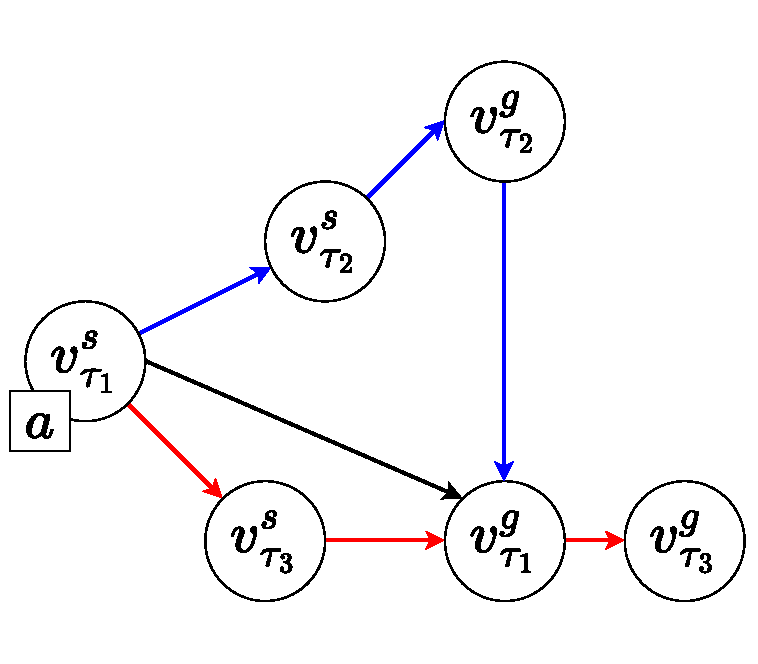
\includegraphics[width=0.5\linewidth]{Fig/carpooling.pdf}
  \caption{The impact of co-passenger tasks}
  \label{fig:carpooling}
  \Description{The impact of co-passenger tasks}
\end{figure}

\begin{example}[Co-passenger tasks]
As shown as in Figure~\ref{fig:carpooling}, there is an agent, $a$, 
and three tasks, $\tau_{1}$, $\tau_{2}$ and $\tau_{3}$.
The agent $a$ is located at pickup location of $\tau_{1}$.
The blue lines are the best schedule for agent $a$ to complete $\tau_{1}$ and $\tau_{2}$.
The red lines are the best schedule for agent $a$ to complete $\tau_{1}$ and $\tau_{3}$.
When we allocate $\tau_{1}$ and $\tau_{2}$ to the agent $a$,
the agent $a$ needs to take the blue paths to complete $\tau_{1}$ and $\tau_{2}$ by greedy strategy,
and it will not impact the completion time of $\tau_{2}$ but lengthen the completed time of $\tau_{1}$.
Howerver, if we allocate $\tau_{1}$ and $\tau_{3}$ to the agent $a$, 
$a$ needs to take the red paths to complete $\tau_{1}$ and $\tau_{3}$.
While it also lengthens the completed time of $\tau_{1}$, 
it is obvious that $\tau_3$ has less of an effect on $\tau_1$ as compared to $\tau_{2}$.
Therefore, we need to consider the impact of "co-passenger" tasks when allocating tasks to agents.
\end{example}


\begin{figure}[htbp]
  \centering
  \subfigure[$S^1_{i,j}$]{
    \label{fig:schedule1}
    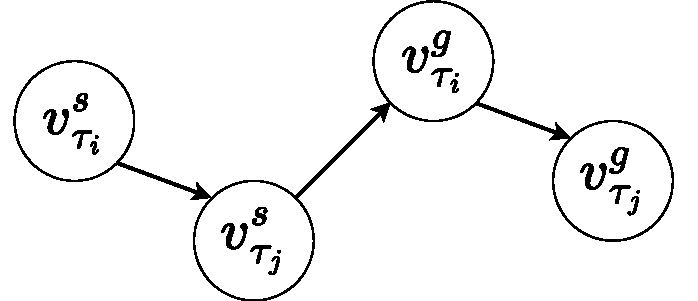
\includegraphics[width=0.4\linewidth]{Fig/path1.pdf}}
  \subfigure[$S^2_{i,j}$]{
    \label{fig:schedule2}
    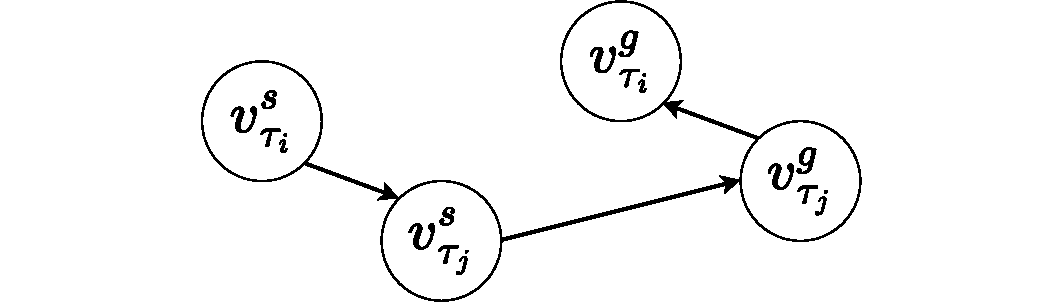
\includegraphics[width=0.4\linewidth]{Fig/path3.pdf}}
  \subfigure[$S^3_{i,j}$]{
    \label{fig:schedule3}
    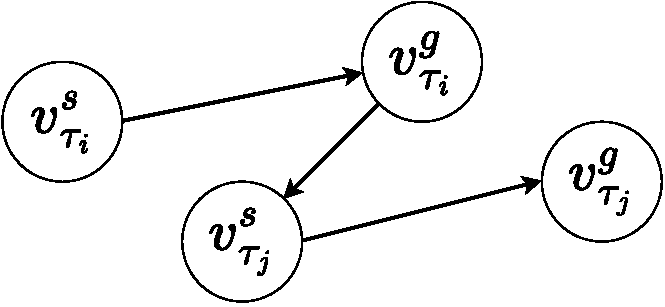
\includegraphics[width=0.4\linewidth]{Fig/path2.pdf}}
  \subfigure[$S^4_{i,j}$]{
    \label{fig:schedule4}
    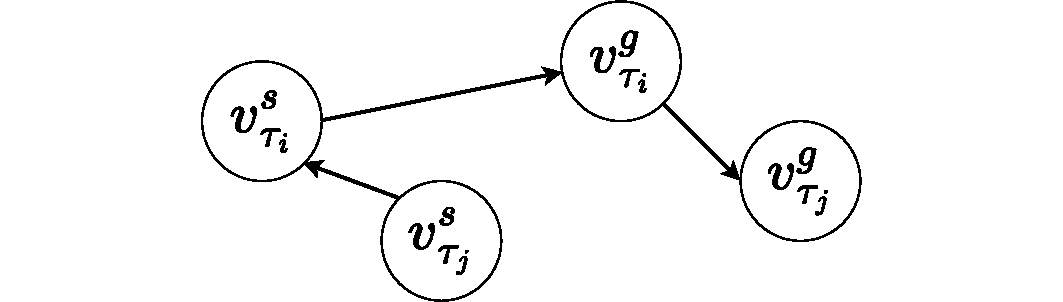
\includegraphics[width=0.4\linewidth]{Fig/path4.pdf}}
  \subfigure[$S^5_{i,j}$]{
    \label{fig:schedule5}
    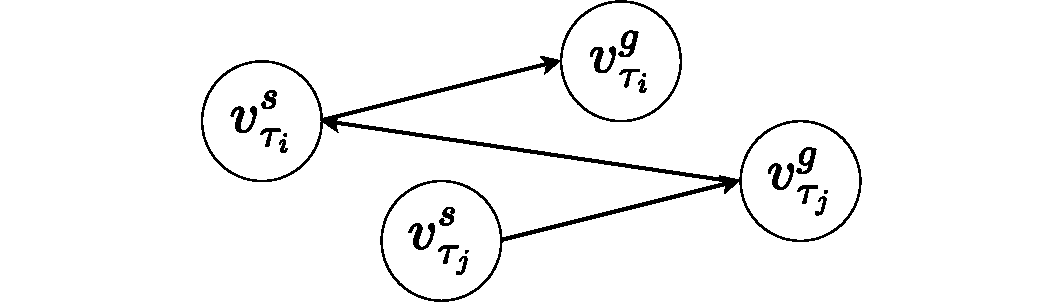
\includegraphics[width=0.4\linewidth]{Fig/path5.pdf}}
  \subfigure[$S^6_{i,j}$]{
    \label{fig:schedule6}
    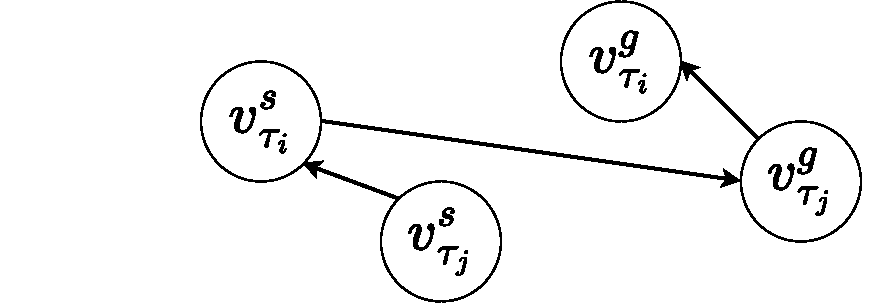
\includegraphics[width=0.4\linewidth]{Fig/path6.pdf}}
  \caption{All possible schedules of two tasks}
  \label{fig:2TP}
  \Description{All possible schedules of two tasks}
\end{figure}

We first analyze the likelihood of carpooling between two tasks.
As shown in Figure~\ref{fig:2TP}, there are 6 schedules to the completion of $\tau_{i}$ and $\tau_{j}$, 
ignoring the location of agent.
The schedules are $S^{1}_{i,j}$, $S^{2}_{i,j}$, $S^{3}_{i,j}$, $S^{4}_{i,j}$, $S^{5}_{i,j}$ and $S^{6}_{i,j}$.
Therefore, we define the carpooling scores between two tasks $\tau_{i}$ and $\tau_{j}$ as follows.

\begin{definition}[Carpooling Scores]
\label{cp2}
    The carpooling scores between two tasks $\tau_{i}$ and $\tau_{j}$ is defined as 
    \begin{eqnarray}
    \label{eq:cp2}
        \delta_{\tau_{i}, \tau_{j}} = min\{Cost(S^{q}_{i,j})\} - 
        dis(v^{g}_{\tau_{i}}, v^{s}_{\tau_{i}}) - dis(v^{g}_{\tau_{j}}, v^{s}_{\tau_{j}})
        % q \in \{1, 2, 3, 4, 5, 6\}
    \end{eqnarray}
    where $q \in [1, 6] \wedge q \in \mathbb{N_+}$. $\delta_{i,j}$ is difference 
    between the best schedule of two tasks 
    and the sum of the distances between the pickup and delivery locations of the two tasks.
    The small $\delta_{i,j}$ indicates that $\tau_{i}$ and $\tau_{j}$ being executed by the same agent
    has less impact on each other's completed time, which can efficiently optimize ${ST}$.
\end{definition}

Howerver, in this paper, we focus on multi-load agents, 
which can carry multiple tasks simultaneously, not just two tasks.
Therefore, we need to consider the carpooling scores between multiple tasks.
It is worth noting that we cannot find the best schedule to complete multiple tasks, 
which is a NP-hard problem.
Therefore, we propose a novel method to schedule there tasks.
Then, we evaluate the upper bound on the cost of the schedule of multiple tasks.
Finally, we quantify the carpooling scores between multiple tasks.

We first introduce the novel schedule method.
As shown in Figure~\ref{fig:K-taskgroup}, there is a set of task $\Gamma_K$, 
which contains K tasks, $\tau_{1}$, $\tau_{2}$, ..., $\tau_{K}$.
The schedule $S'_{\Gamma_K}$ of K tasks is shown in Figure~\ref{fig:KTG-path}.
This schedule starts at the pickup location of a task in $\Gamma_K$, 
then goes to the pickup location of other tasks in $\Gamma_K$, 
and finally to the delivery location of all tasks in $\Gamma_K$.
%% 感觉怪
More significantly, in $S'_{\Gamma_K}$,
the path between two pickup or delivery locations about two tasks in $\Gamma_K$ 
is is part of paths of the best schedules of two tasks.
For example, if path $v^{s}_{\tau_{i}}$ and $v^{s}_{\tau_{j}}$ is part of the best schedule of two tasks,
then the path between $v^{s}_{\tau_{i}}$ and $v^{s}_{\tau_{j}}$ is part of the path of $S'_{\Gamma_K}$.
Therefore, Theorem~\ref{thm:TaskGroupCost} is proposed to find the upper bound on cost of the schedule of $S'_{\Gamma_K}$,
and prove it.

\begin{figure}[ht]
  \centering
  \subfigure[$\Gamma_K$]{
    \label{fig:K-taskgroup}
    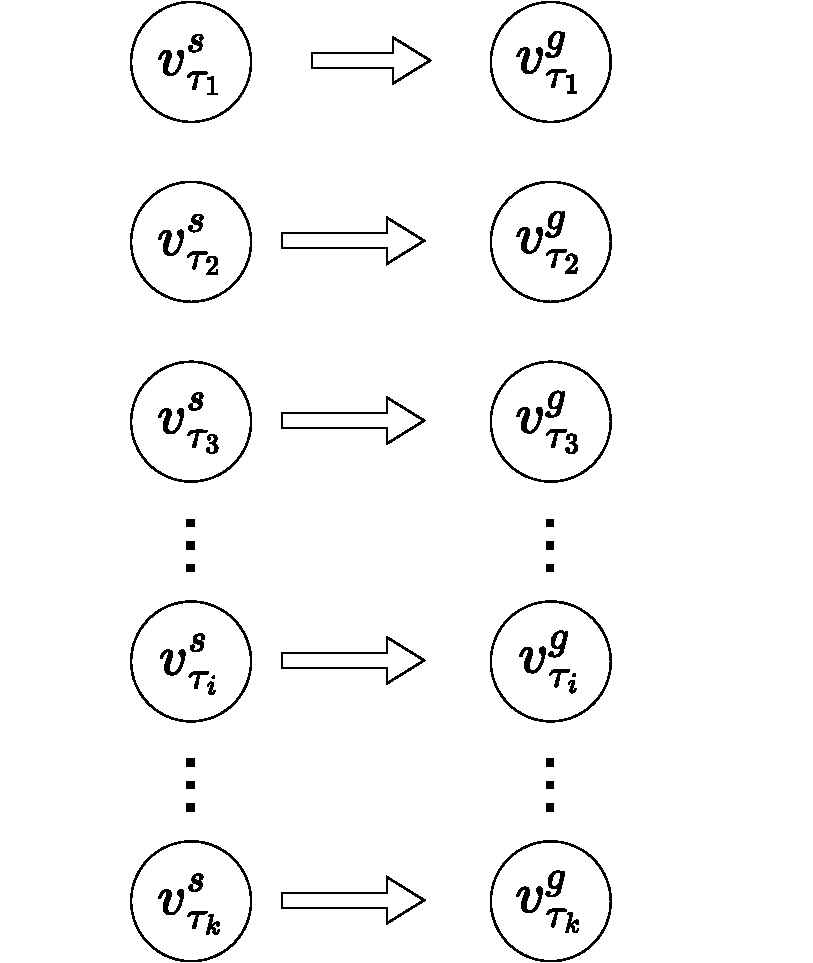
\includegraphics[width=0.4\linewidth]{Fig/k-tasks.pdf}}
  \subfigure[Schedule of $\Gamma_K$]{
    \label{fig:KTG-path}
    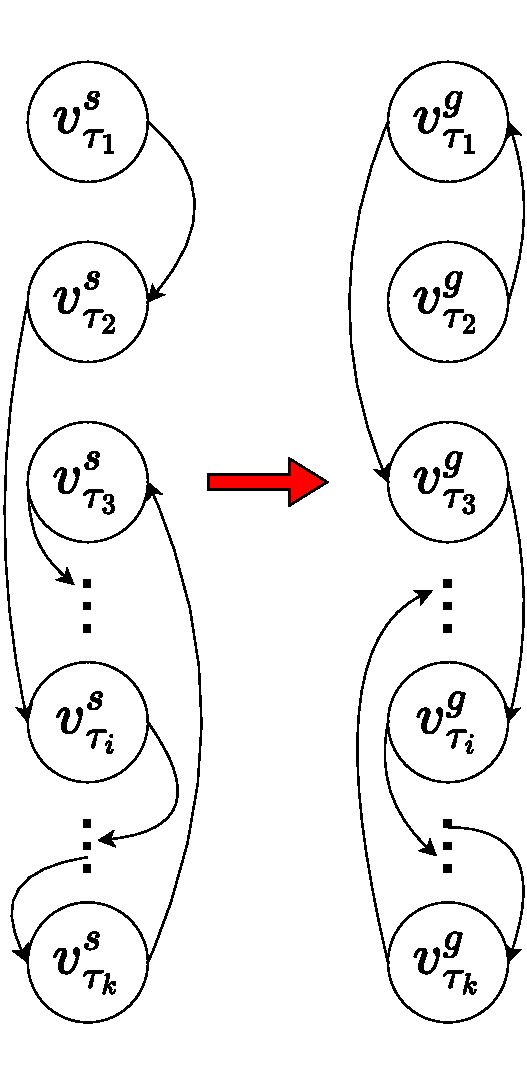
\includegraphics[width=0.4\linewidth]{Fig/Path-KT.pdf}}
  \caption{Schedule of K Tasks}
  \label{PKT}
  \Description{Schedule of K Tasks}
\end{figure}

\begin{theorem}
    \label{thm:TaskGroupCost}
    Given a set of tasks $\Gamma_K$, there exists a schedule $S'_{\Gamma_K}$ shown in Figure~\ref{fig:KTG-path} 
    such that the following bound holds.
    
    \begin{eqnarray}
        \label{eq:tgc}
        Cost(S'_{\Gamma_K}) \leq 2 {\ast} \sum_{\tau_i \in \Gamma_K}{dis(v^{s}_{\tau_i}, v^{g}_{\tau_i})} 
        + 2{\ast}(K-1)\delta
    \end{eqnarray}
    where $\delta$ is the carpooling scores between two tasks.
\end{theorem}

\begin{figure}[ht]
  \centering
  \subfigure[Tournament]{
  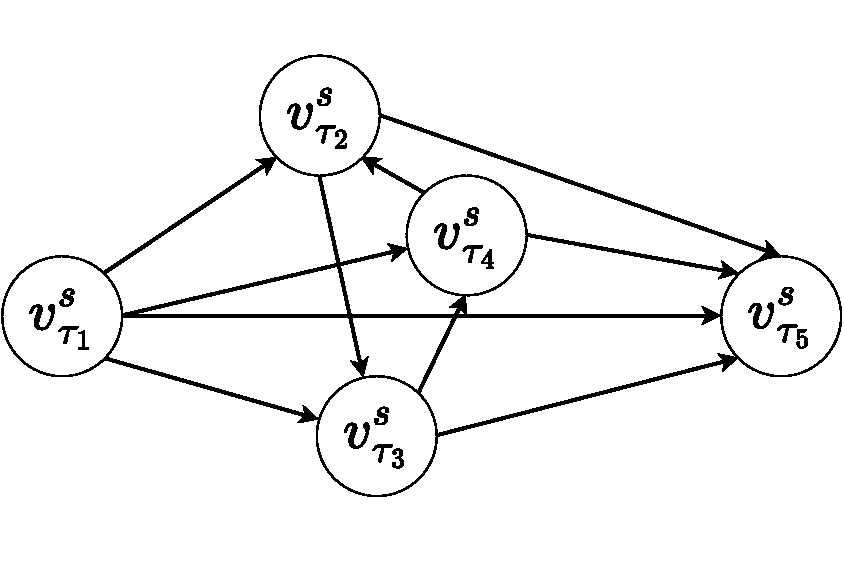
\includegraphics[width=0.3\linewidth]{Fig/tournament.pdf}
  \label{fig:tournament}}
  \subfigure[SCC]{
  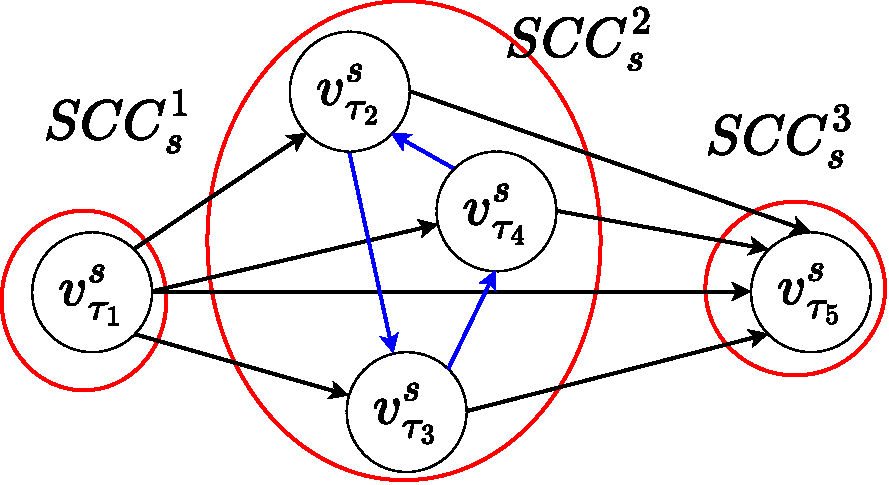
\includegraphics[width=0.3\linewidth]{Fig/SCCs.pdf}
  \label{SCC}}
  % \subfigure[suodian]{
  % 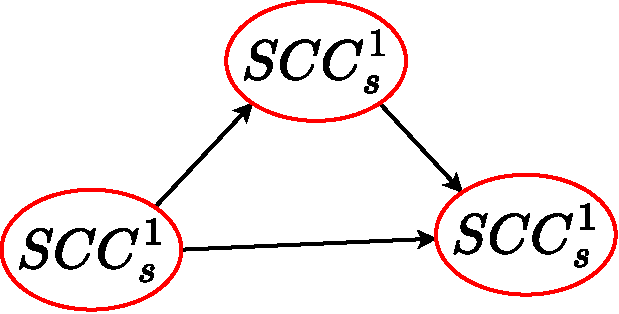
\includegraphics[width=0.4\linewidth]{Fig/suodian.pdf}
  % \label{fig:suodian}}
  \subfigure[topologize]{
  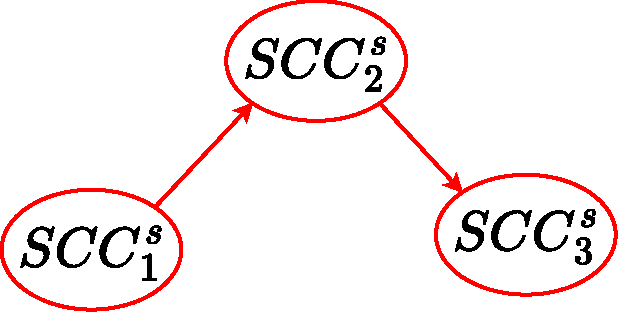
\includegraphics[width=0.3\linewidth]{Fig/topologize.pdf}
  \label{fig:topologize}}
  \caption{The tournament and SCC}
  \label{fig:tournament-SCC}
  \Description{The tournament and SCC}
\end{figure}

\begin{proof}
    Firstly, we need to prove that there is a path to complete $\Gamma_K$.
    As shown in Figure~\ref{fig:KTG-path},
    the schedule first connects the pickup locations of all tasks in $\Gamma_K$,
    then connects the delivery locations of all tasks in $\Gamma_K$.
    Focusing on the pickup locations set of $\Gamma_K$
    and connecting the pickup locations,
    we can get a tournament~\cite{enwiki:1234378036}, 
    which is a directed graph with exactly one edge between each two vertices, 
    in one of the two possible directions.
    As shown in Figure~\ref{fig:tournament}, 
    there are 5 pickup locations,
    and a path between each two locations.
    Accroding to the definition of tournament,
    there is a Hamiltonian path in the tournament~\cite{enwiki:1234378036},
    that means there exists a path to connect all pickup locations of $\Gamma_K$.
    Similarly, there is a path to connect all delivery locations of $\Gamma_K$.
    Then, we need to find a path to connect the pickup locations and delivery locations.
    Therefore, we introduce the Strongly Connected Component (SCC)~\cite{SCC},
    which is a subgraph that is strongly connected.
    As shown in Figure~\ref{SCC},
    $v^{s}_{\tau_{2}}$, $v^{s}_{\tau_{3}}$ and $v^{s}_{\tau_{4}}$ combine  to form a SCC
    where there is a path between each two locations.
    When we shrink the SCC to a single vertex 
    and focus on the last SCC of the pickup locations and first SCC of the delivery locations,
    we can always find two locations, $v^{s}_{\tau_{i}}$ and $v^{g}_{\tau_{j}}$, in two SCCs respectively,
    which connects the pickup locations and delivery locations.
    Moreover, $dis(v^{g}_{\tau_{j}}, v^{s}_{\tau_{i}})$ is less than or equal to 
    $dis(v^{g}_{\tau_{j}}, v^{s}_{\tau_{j}}) + dis(v^{g}_{\tau_{i}}, v^{s}_{\tau_{i}})$.
    (The proof is shown in appendix).
    % proof that in appendix

    Secondly, we need to evaluate the cost of the path.
    In the beginning, we evaluate the cost of the path between the pickup locations.
    $dis(v^{s}_{\tau_{j}}, v^{s}_{\tau_{i}})$ is the distance 
    between the pickup locations of $\tau_{i}$ and $\tau_{j}$,
    and all possible schedules of two tasks are shown in Figure~\ref{fig:2TP}.
    If the best schedule of two tasks is $S^{1}_{i,j}$,
    we can get Equation~\ref{eq:dis1}.
    \begin{eqnarray}
      \label{eq:dis1}
      Cost(S^{1}_{i,j}) &=& dis(v^s_{\tau_j}, v^s_{\tau_i})+dis(v^g_{\tau_i}, v^s_{\tau_j})
      +dis(v^g_{\tau_j}, v^g_{\tau_i}) \nonumber \\
      % dis(v^g_{\tau_j}, v^s_{\tau_j}) + dis(v^g_{\tau_i}, v^s_{\tau_i}) + \delta_{\tau_i, \tau_j}
      & \geq & dis(v^s_{\tau_j}, v^s_{\tau_i})+ dis(v^g_{\tau_j}, v^s_{\tau_j})\\
      \label{eq:dis2}
      dis(v^g_{\tau_i}, v^s_{\tau_i})+\delta_{\tau_i, \tau_j} &\geq& dis(v^s_{\tau_j}, v^s_{\tau_i})
    \end{eqnarray}
    Then, based on this Definition~\ref{cp2}, we can get Equation~\ref{eq:dis2}.
    Finally, we check all the possible schedules of two tasks in Figure~\ref{fig:2TP},
    and we ensure the Equation~\ref{eq:dis2} holds.
    Similarly, we can evaluate the cost of the path between the delivery locations
    by the same method and get Equation~\ref{eq:dis3}. (The proof is shown in appendix).
    \begin{eqnarray}
      \label{eq:dis3}
      dis(v^{g}_{\tau_{j}}, v^{s}_{\tau_{j}})+ \delta_{i,j} &\geq& dis(v^{g}_{\tau_{j}}, v^{g}_{\tau_{i}})
    \end{eqnarray}
    Therefore, we can evaluate the cost of the path between the pickup locations and delivery locations.
    The cost of paths in pickup locations less than or equal to 
    $\sum_{\tau_i \in {\Gamma_K \setminus \tau_i}}{dis(v^{s}_{\tau_i}, v^{g}_{\tau_i})}$ + $(K-1)\delta$,
    which $\tau_i$ is the last pickup location in $S'_{\Gamma_K}$.
    The cost of paths in delivery locations less than or equal to
    $\sum_{\tau_i \in \Gamma_K \setminus \tau_j}{dis(v^{s}_{\tau_i}, v^{g}_{\tau_i})}$ + $(K-1)\delta$,
    which $\tau_j$ is the first delivery location in $S'_{\Gamma_K}$.
    The cost of the path $dis(v^{g}_{\tau_{j}}, v^{s}_{\tau_{i}})$, 
    which connects the pickup locations and delivery locations in $S'_{\Gamma_K}$,
    is less than or equal to $dis(v^{g}_{\tau_{j}}, v^{s}_{\tau_{j}}) + dis(v^{g}_{\tau_{i}}, v^{s}_{\tau_{i}})$.
    Therefore, the cost of the schedule is less than or equal to 
    $2 {\ast} \sum_{\tau_i \in \Gamma_K}{dis(v^{s}_{\tau_i}, v^{g}_{\tau_i})} + 2{\ast}(K-1)\delta$.
\end{proof}

Next, we can introduce the Get Carpooling Scores Algorithm (GCS)
to quantify the carpooling scores between multiple tasks $\Gamma_K$ as follows.
Accroding to the Theorem~\ref{thm:TaskGroupCost},
to be more efficient,
we fisrt use Tarjan algorithm~\cite{tarjan1972depth} to get the SCCs of the set of tasks,
and topologize it to get chain of SCC like Figure~\ref{fig:topologize}.
Then, in order to be more precise about $\delta$,
we calculate the carpooling scores in each SCC by Equation~\ref{eq:inSCC},
and between two SCCs by Equation~\ref{eq:betweenSCC}.
Finally, we get the carpooling scores between two task groups by Algorithm~\ref{alg:GCS}.
The result of this algorithm is the part of Theorem~\ref{thm:TaskGroupCost}, $2*(K-1)\delta$.
the smaller the result leads to
the lower the upper bound on cost of schedule, and the less the impact between tasks.

\begin{eqnarray}
  \label{eq:inSCC}
    \Delta_{SCC} =\frac{2 {\ast} \sum_{\tau_i \in SCC}{\sum_{\tau_j \in SCC}{\delta_{\tau_i, \tau_j}}} }
    {|SCC|}\\
  \label{eq:betweenSCC}
    \Delta_{SCC_i, SCC_{i+1}} = \frac{\sum_{\tau_i \in SCC_i}{\sum_{\tau_j \in SCC_{i+1}}{\delta_{\tau_i, \tau_j}}} }
    {|SCC^i|{\ast}|SCC^{i+1}|}
\end{eqnarray}
where $SCC$ is the Strongly Connected Component,
$|SCC|$ is the number of tasks in $SCC$.
Equation~\ref{eq:inSCC} is average $\delta$ in $SCC$,
which contains $|SCC|-1$ carpooling scores between tasks.
Equation~\ref{eq:betweenSCC} is average $\delta$ between $SCC_i$ and $SCC_{i+1}$,
which contains one carpooling score between two tasks in $SCC_i$ and $SCC_{i+1}$.


\begin{algorithm}[htbp]
\caption{Get Carpooling Scores Algorithm}
\label{alg:GCS}
\begin{algorithmic}[1]
\Require Set of tasks $\Gamma_K$ %%input
\Ensure Carpooling scores $\Delta_{\Gamma_K}$ %%output
\State Initialize $\Delta_{\Gamma_K} = 0$
\State Call Tarjan algorithm to get $SCC^s$ and $SCC^g$ of $\Gamma_K$
\For {$SCC^s_{i} \in SCC^s$}
    % \State $\Delta_{SCC^s_i} =\frac{2 {\ast} \sum_{\tau_i \in SCC^s_{i}}{\sum_{\tau_j \in SCC^s_{i}}{\delta_{\tau_i, \tau_j}}} }
    % {|SCC^s_{i}|}$
    \State Get $\Delta_{SCC^s_i}$ by Equation~\ref{eq:inSCC}
    \If {$SCC^s_i$ is not last SCC}
        % \State $\Delta_{SCC^s_i, SCC^s_{i+1}} = \frac{\sum_{\tau_i \in SCC^s_i}{\sum_{\tau_j \in SCC^s_{i+1}}{\delta_{\tau_i, \tau_j}}} }
        % {|SCC^s_i|{\ast}|SCC^s_{i+1}|}$
        \State Get $\Delta_{SCC^s_i, SCC^s_{i+1}}$ by Equation~\ref{eq:betweenSCC}
    \EndIf
    \State $\Delta_{\Gamma_K} += \Delta_{SCC}$ + $\Delta_{SCC^s_i, SCC^s_{i+1}}$
\EndFor
\State Do the same for $SCC^g$
\State \Return $\Delta_{\Gamma_K}$
\end{algorithmic}
\end{algorithm}

\textbf{Algorithm Detail:} 
The pseduo-code of Get Carpooling Scores Algorithm is shown in Algorithm~\ref{alg:GCS},
where the input is a set of tasks $\Gamma_K$ containing K tasks,
and the output is the carpooling scores $\Delta_{\Gamma_K}$.
First, we initialize $\Delta_{\Gamma_K}$ to 0.
Then, we call Tarjan algorithm~\cite{tarjan1972depth} to get the SCCs of $\Gamma_K$ (lines 1-2).
For each SCC, we calculate the carpooling scores in the SCC and between two SCCs (lines 3-10).
Finally, we return the carpooling scores $\Delta_{\Gamma_K}$ (line 11).

\textbf{Analysis:}
The time complexity of GCS algorithm is $O(K^2)$,
where $K$ is the number of tasks in $\Gamma_K$.
The Tarjan algorithm~\cite{tarjan1972depth} has a time complexity of $O(|V|+|E|)$,
where $|V|$ is the number of vertices and $|E|$ is the number of edges.
Therefore, $O(K^2)$ is the time complexity of call Tarjan algorithm to get the SCCs of $\Gamma_K$ (line 2).
The time complexity of calculating the carpooling scores in each SCC and between SCCs is $O(K)$ (lines 3-10).
Therefore, the time complexity of GCS algorithm is $O(K^2)$.

\subsection{K-Capacity Hierarchical Clustering}
% diff between task group and single task
Based on Theorem~\ref{thm:TaskGroupCost},
we can quantify the carpooling scores between multiple tasks.
Howerver, the schedule of multiple tasks needs to go to the pickup locations of all tasks first.
In MLAPD problem, the maximum load capacity of the agent limits 
the size of the set of tasks that we can quantify the carpooling scores.
Therefore, the K-Capacity Hierarchical Clustering Algorithm (KCHC)
is proposed to divide the set of tasks into groups by carpooling scores,
which contain at most K tasks.
K is the maximum load capacity of the agent.
The KCHC algorithm is shown in Algorithm~\ref{alg:KCHC}.

\begin{algorithm}[htbp]
\caption{K-Capacity Hierarchical Clustering Algorithm}
\label{alg:KCHC}

\begin{algorithmic}[1]
\Require Set of tasks $\Gamma$, the max capacity of agents $K$ %%input
\Ensure Set of task groups ${\Pi}$ %%output
\State Initialize ${\Pi} = \emptyset$
\For {$\tau_{i} \in \Gamma$}
    \State Treat $\tau_{i}$ as a task group $\Gamma_{i}$, and add $\Gamma_{i}$ into ${\Pi}$
    \For{$\Gamma_j \in \Pi$ and $\tau_j \in \Gamma_j$}
        \State $\Delta_{\Gamma_i \cup \Gamma_j} = \delta_{\tau_i, \tau_j}$
    \EndFor
\EndFor
\While{$\Pi$ has changed}
    \State Select minimum carpooling scores $\Delta_{\Gamma_p \cup \Gamma_q}$ from $\Pi$
    \State Merge $\Gamma_p$ and $\Gamma_q$ into $\Gamma_{p+q}$
    \State Remove $\Gamma_p$ and $\Gamma_q$ from $\Pi$ and add $\Gamma_{p+q}$ into $\Pi$
    \For{$\Gamma_j \in \Pi$}
        \If {$|\Gamma_j| + |\Gamma_{p+q}| \leq K$}
            % \State $\Gamma = \Gamma_{p+q} \cup \Gamma_j$
            \State Get $\Delta_{\Gamma_{p+q} \cup \Gamma_j}$ by Algorithm~\ref{alg:GCS}
        \EndIf
    \EndFor
\EndWhile
\State \Return $\Pi$
\end{algorithmic}
\end{algorithm}

\textbf{Algorithm Detail:}
The pseduo-code of K-Capacity Hierarchical Clustering Algorithm is shown in Algorithm~\ref{alg:KCHC},
where the input is a set of tasks $\Gamma$ and the max capacity of agents $K$,
and the optput is a set of task groups $\Pi$.
First, we initialize $\Pi$ to an empty set (line 1).
Then, we treat each task as a task group and add it to $\Pi$,
and calculate the carpooling scores between each pair of task groups (lines 2-7).
Next, we iteratively merge the task groups with the minimum carpooling scores.
If the size of the merged task group is less than or equal to $K$,
we merge the task groups and calculate the carpooling scores between them,
and calculate the carpooling scores between the merged task group and other task groups (lines 8-18).
Finally, we return the set of task groups $\Pi$ (line 19).

\textbf{Analysis:}
If the number of tasks in $\Gamma$ is $N$,
the time complexity of KCHC algorithm is $O(N^2)$.
The time complexity of calculating the carpooling scores between each pair of task groups is $O(N^2)$ (lines 2-7).
The time complexity of merging the task groups is $O(N^2)$ (lines 8-18).
In each iteration, we merge two task groups, calculate the carpooling scores between the merged task group and other task groups,
and the number of task groups is reduced by 1,
so we need to iterate $(N-N/K)$ times at most 
and calculate the carpooling scores with $N$ task groups at most.
Therefore, the time complexity of KCHC algorithm is $O(N^2)$.


\subsection{Task Group Allocation Algorithm}

% 说明为什么要搞task group allocation

Before we introduce the Task Group Allocation Algorithm,
we first define the detour cost of the schedule of agent $a$ to complete $\Gamma$,
which is the difference between the cost of the schedule and the sum of the distances between the pickup and delivery locations of the tasks in $\Gamma$.
The detour cost is used to evaluate the rationality of the schedule of agent $a$ to complete $\Gamma$.
\begin{eqnarray}
  \label{eq:DCost}
  DCost(S_{\Gamma_{a}}) = Cost(S_{\Gamma_{a}}) - \sum_{\tau_i \in \Gamma_a}{dis(v^{s}_{\tau_i}, v^{g}_{\tau_i})}
\end{eqnarray}
where $S_{\Gamma_{a}}$ is the schedule of agent $a$ to complete $\Gamma$.
Therefore, we introduce the Get Schedule of Task Group Algorithm (GSTG) 
to the schedule of task group by Equation~\ref{eq:DCost}.

Next, we introduce Get Schedule of Task Group (GSTG) Algorithm 
to get the schedule of task group by the detour cost.
The GSTG algorithm is shown in Algorithm~\ref{alg:ScheduleTG}.
\begin{algorithm}[htbp]
\caption{Get Schedule of Task Group}
\label{alg:ScheduleTG}
\begin{algorithmic}[1]
\Require Set of tasks $\Gamma$, Agent $a$ %%input
\Ensure The detour cost of schedule $DCost({S_{\Gamma}})$ %%output
\State Initialize $Cost({S_{\Gamma}}) = 0$
\While {$\Gamma$ is not empty}
  \For {$\tau_i \in \Gamma$, adjacent locations $v_{i}$ and $v_{j}$ in $S_{\Gamma_a}$}
      \State Insert $v^s_{\tau_i}$, $v^g_{\tau_i}$ between $v_{i}$ and $v_{j}$, respectively
      \State Calculate the detour cost $DCost(S_{\Gamma_{a}})$.
  \EndFor
  \State Select task $\tau$ with minimum detour cost
  \State Remove $\tau$ from $\Gamma$
\EndWhile
\State \Return $DCost({S_{\Gamma}})$
\end{algorithmic}
\end{algorithm}

\textbf{Algorithm Detail:}
The pseduo-code of Get Schedule of Task Group Algorithm is shown in Algorithm~\ref{alg:ScheduleTG},
where the input is a set of tasks $\Gamma$ and an agent $a$,
and the output is the detour cost of the schedule $DCost({S_{\Gamma}})$.
First, we initialize the cost of the schedule $Cost({S_{\Gamma}})$ to 0 (line 1).
Then, we iteratively insert the pickup and delivery locations of tasks in $\Gamma$ into the schedule $S_{\Gamma_a}$,
and calculate the detour cost of the schedule $DCost(S_{\Gamma_{a}})$ (lines 2-6).
Select the task with the minimum detour cost and remove it from $\Gamma$,
until $\Gamma$ is empty (lines 7-9).
Finally, we return the detour cost of the schedule $DCost({S_{\Gamma}})$ (line 10).

% \textbf{Analysis:}
% If the number of tasks in $\Gamma$ is $N$,
% the time complexity of GSTG algorithm is $O(N^2)$.
% The time complexity of inserting the pickup and delivery locations of tasks in $\Gamma$ into the schedule $S_{\Gamma_a}$ is $O(N^2)$ (lines 2-6).
% The time complexity of selecting the task with the minimum detour cost and removing it from $\Gamma$ is $O(N)$ (lines 7-9).
% Therefore, the time complexity of GSTG algorithm is $O(N^2)$.

Then, we allocate task groups to agents.
Howerver, we cannot indirectly allocate task groups to agents,
since we do not consider the location of agents, while dividing tasks into groups.
It maybe lead to the situation that agents schedule task groups inappropriately.

\begin{figure}[ht]
  \centering
  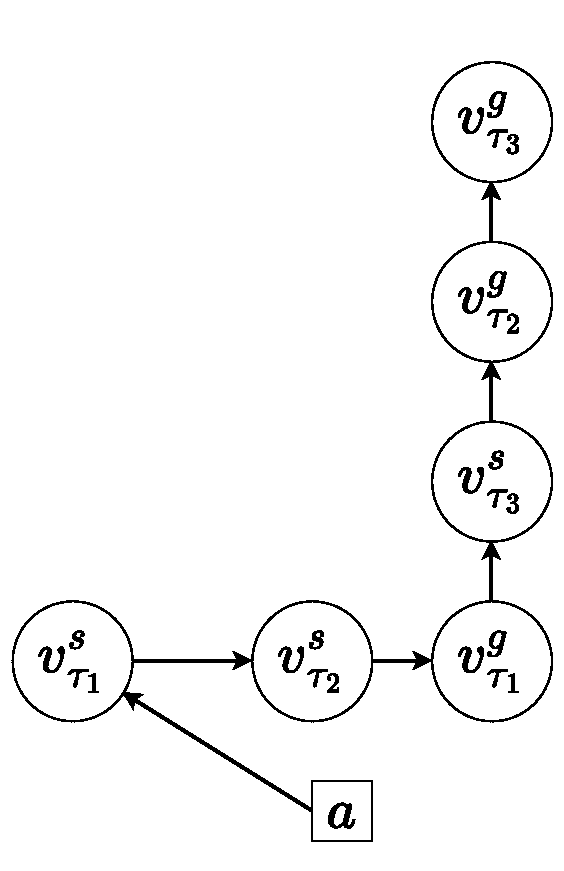
\includegraphics[width=0.3\linewidth]{Fig/A-TG.pdf}
  \caption{The schedule of agent $a$ to complete $\Gamma$}
  \label{fig:agent-taskgroup}
  \Description{The schedule of agent $a$ to complete $\Gamma$}
\end{figure}

\begin{example}

  As shown in Figure~\ref{fig:agent-taskgroup},
  there is an agent, $a$, and a task group $\Gamma$, which contains three tasks, $\tau_{1}$, $\tau_{2}$ and $\tau_{3}$.
  The black lines are the best schedule $S_\Gamma$ of $a$ to complete $\Gamma$.
  Obviously, in black lines, $a$ requires a detour to pickup location of $\tau_{1}$,
  which is irrational schedule.
  

\end{example}

Therefore, to consider the location of agents,
we split the task group $\Gamma$ into multiple subgroups,
\begin{eqnarray}
  \label{eq:split}
  \Pi_{\Gamma} = \{ \forall \Gamma_i | \Gamma_i \subset \Gamma \}
\end{eqnarray}
where $\Pi_{\Gamma}$ is the set of subgroups of $\Gamma$.


Based on there,
we propose the Task Group Allocation Algorithm to allocate task groups to agents.


\begin{algorithm}[htbp]
\caption{Task Group Allocation Algorithm}
\label{alg:TGA}
\begin{algorithmic}[1]
\Require Set of tasks $\Gamma$, set of agents $A$ %%input
\Ensure Schedules of all agents %%output
\State $K$ = the max capacity of agents
% \State $\Pi$ = K-Capacity Hierarchical Clustering Algorithm($\Gamma$, $K$)
\State Get task groups $\Pi$ by Algorithm~\ref{alg:KCHC}
\For {$\Gamma \in \Pi$}
    \State Get $\Pi_{\Gamma}$ by Equation~\ref{eq:split}
    \State ${\tilde{\Pi}}$ extends $\Pi_{\Gamma}$
\EndFor
\For {$a_i \in A$, $\Gamma_j \in {\tilde{\Pi}}$}
    \State Get detour cost $DCost(S_{\Gamma_{a_i}})$ by Algorithm~\ref{alg:ScheduleTG}
\EndFor
\While {${\tilde{\Pi}}$ is not empty}
    \State Select agent $a$ and task group $\Gamma$ with minimum detour cost
    \State Remove $\Gamma$ and $\{\forall \Gamma'| \Gamma'\cap \Gamma \neq \phi \} $ from ${\tilde{\Pi}}$
    \State Update the schedule of $a$ to complete $\Gamma$
    \For {$\Gamma' \in {\tilde{\Pi}}$}
        \State Update the detour cost of schedule of $a$ to complete $\Gamma'$
    \EndFor
\EndWhile
\State \Return Schedules of all agents
\end{algorithmic}
\end{algorithm}

\textbf{Algorithm Detail:}
The pseduo-code of Task Group Allocation Algorithm is shown in Algorithm~\ref{alg:TGA},
where the input is a set of tasks $\Gamma$ and a set of agents $A$,
and the output is the schedules of all agents.
First, we initialize the maximum load capacity of agents $K$,
and then divide the set of tasks $\Gamma$ into task groups by the K-Capacity Hierarchical Clustering Algorithm (lines 1-2).
For each task group $\Gamma$, we split it into subgroups by Equation~\ref{eq:split}
and extend the set of subgroups $\Pi_{\Gamma}$ (lines 3-6).
Then, we calculate the detour cost of the schedule of each agent to complete each task group by the GSTG Algorithm (lines 7-9).
Next, we iteratively select the agent and task group with the minimum detour cost,
remove the task group and the task groups that intersect with it from $\tilde{\Pi}$,
and update the schedule of the agent to complete the task group (lines 11-13).
Moreover, we need to update the detour cost of the schedule of the agent to complete the remaining task groups (lines 14-16).
Finally, we return the schedules of all agents (line 18).

\textbf{Analysis:}
If the number of tasks in $\Gamma$ is $N$ and the number of agents is $M$,
the time complexity of TGA algorithm is $O(N^2)$.
The time complexity of dividing the set of tasks $\Gamma$ into task groups by the K-Capacity Hierarchical Clustering Algorithm is $O(N^2)$ (lines 1-2).
Then, we split each task group into subgroups and extend the set of subgroups $\Pi_{\Gamma}$,
which contains at most $K*N$ task groups (lines 3-6).
Due to $K$ is a constant,
the time complexity of calculating the detour cost of the schedule of each agent 
to complete each task group is $O(N*M)$ (lines 7-9).
Next, $O(N)$ is the time complexity of selecting the agent and task group with the minimum detour cost,
removing the task group and the task groups that intersect with it from $\tilde{\Pi}$,
and updating the schedule of the agent to complete the task group (lines 11-13).
Moreover, the time complexity of updating the detour cost of the schedule of the agent to complete the remaining task groups is $O(N*N)$ (lines 14-16).
Therefore, the time complexity of TGA algorithm is $O(N^2)$.


\section{EXPERIMENTAL ANALYSIS}
\label{sec:experiment}
\subsection{Experimental Settings}
\begin{figure}[htbp]
  \centering
  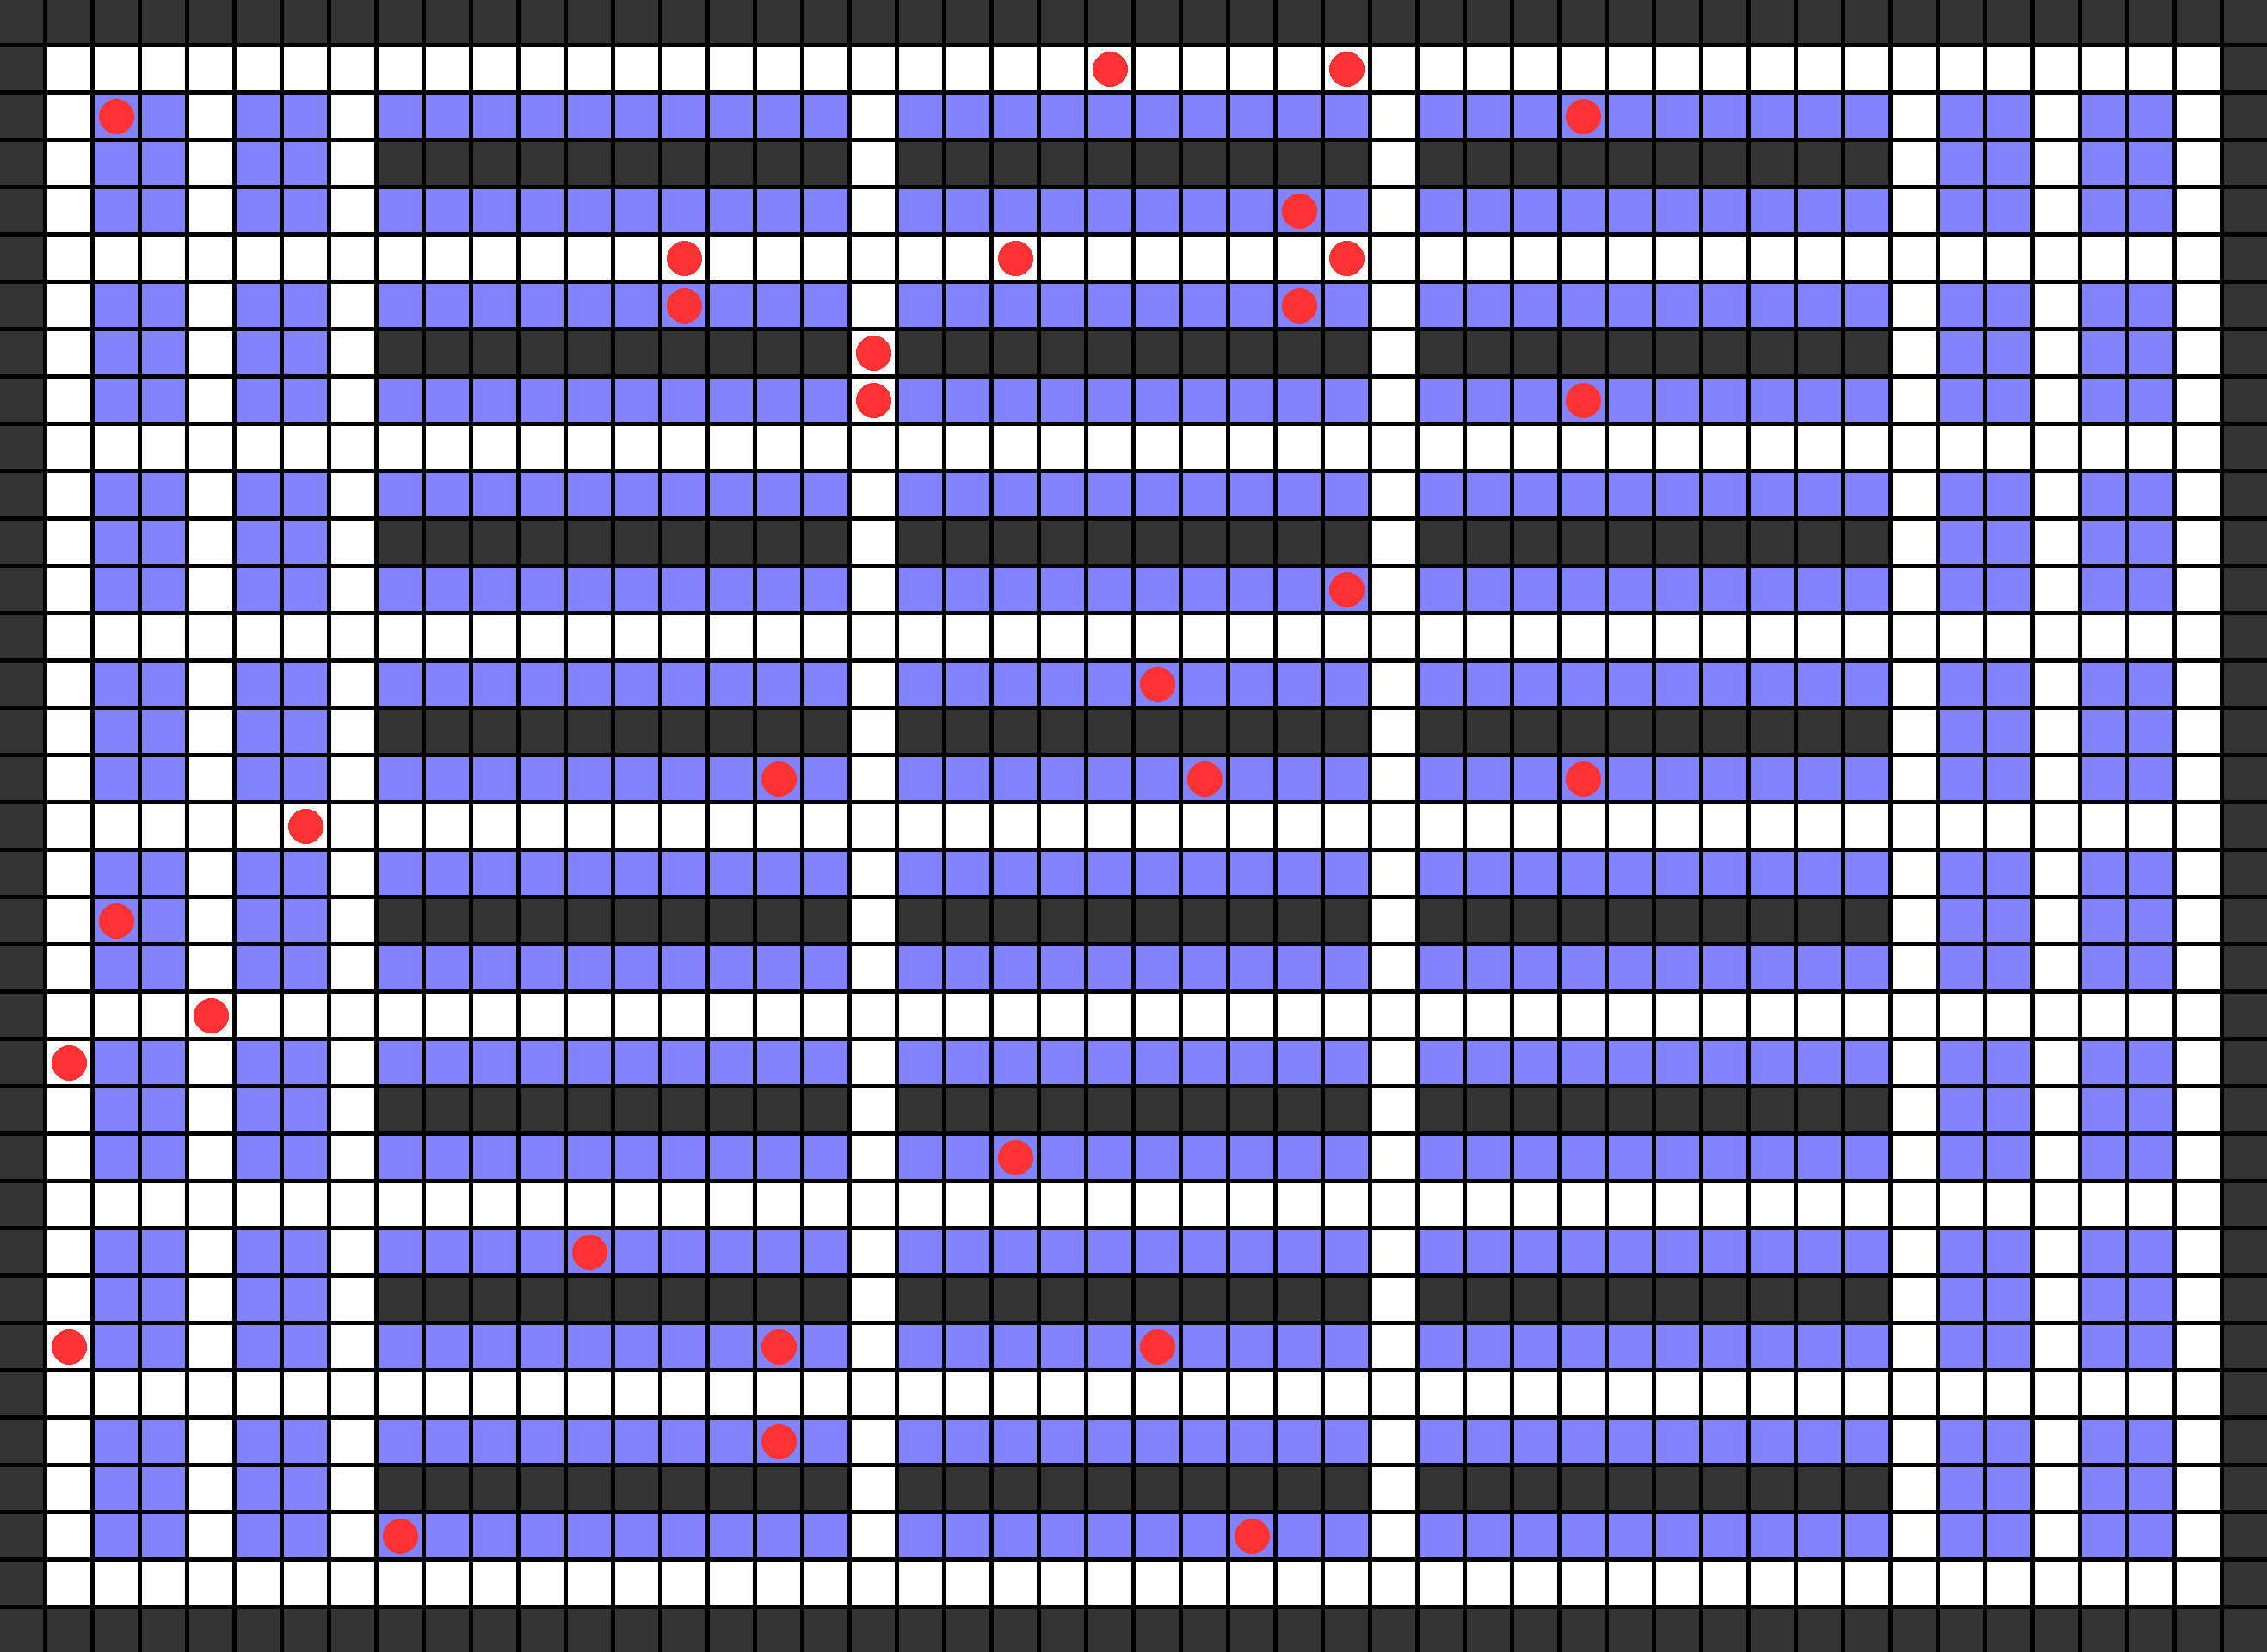
\includegraphics[width=0.5\linewidth]{Fig/map.png}
  \caption{The map}
  \label{fig:map}
  \Description{The map}
\end{figure}
In this section, we first introduce the experimental settings,
which include the map, the evaluation metrics, and the compared algorithms.
Then, we present the experimental results and analyze the performance of the proposed algorithm.

\begin{table}[htbp]
  \centering
  \caption{Experimental Settings}
  \label{tab:settings}
  \begin{tabular}{c|c}
    \toprule
    Parameter & Value \\
    \midrule
    Number of tasks & 2k,4k,\textbf{6k},8k,10k\\
    Number of agents & 30,40,\textbf{50},60,70 \\
    Max capacity of agents & 2,\textbf{3},4,5 \\

    \bottomrule
  \end{tabular}
\end{table}


We conduct experiments in a 33$\times$46 grid map~\cite{ma2017lifelong,ma2019lifelong},
which is shown in Figure~\ref{fig:map}.
In Figure~\ref{fig:map}, the black grid is an obstacle,
the blue grid is the pickup location or delivery location of a task,
the white grid is the road,
and the red circle presents an agent.


\begin{figure*}[htbp]
  \centering
  \subfigure[$|\Gamma|$ vs. ST]{
    \label{fig:ep:taskST}
    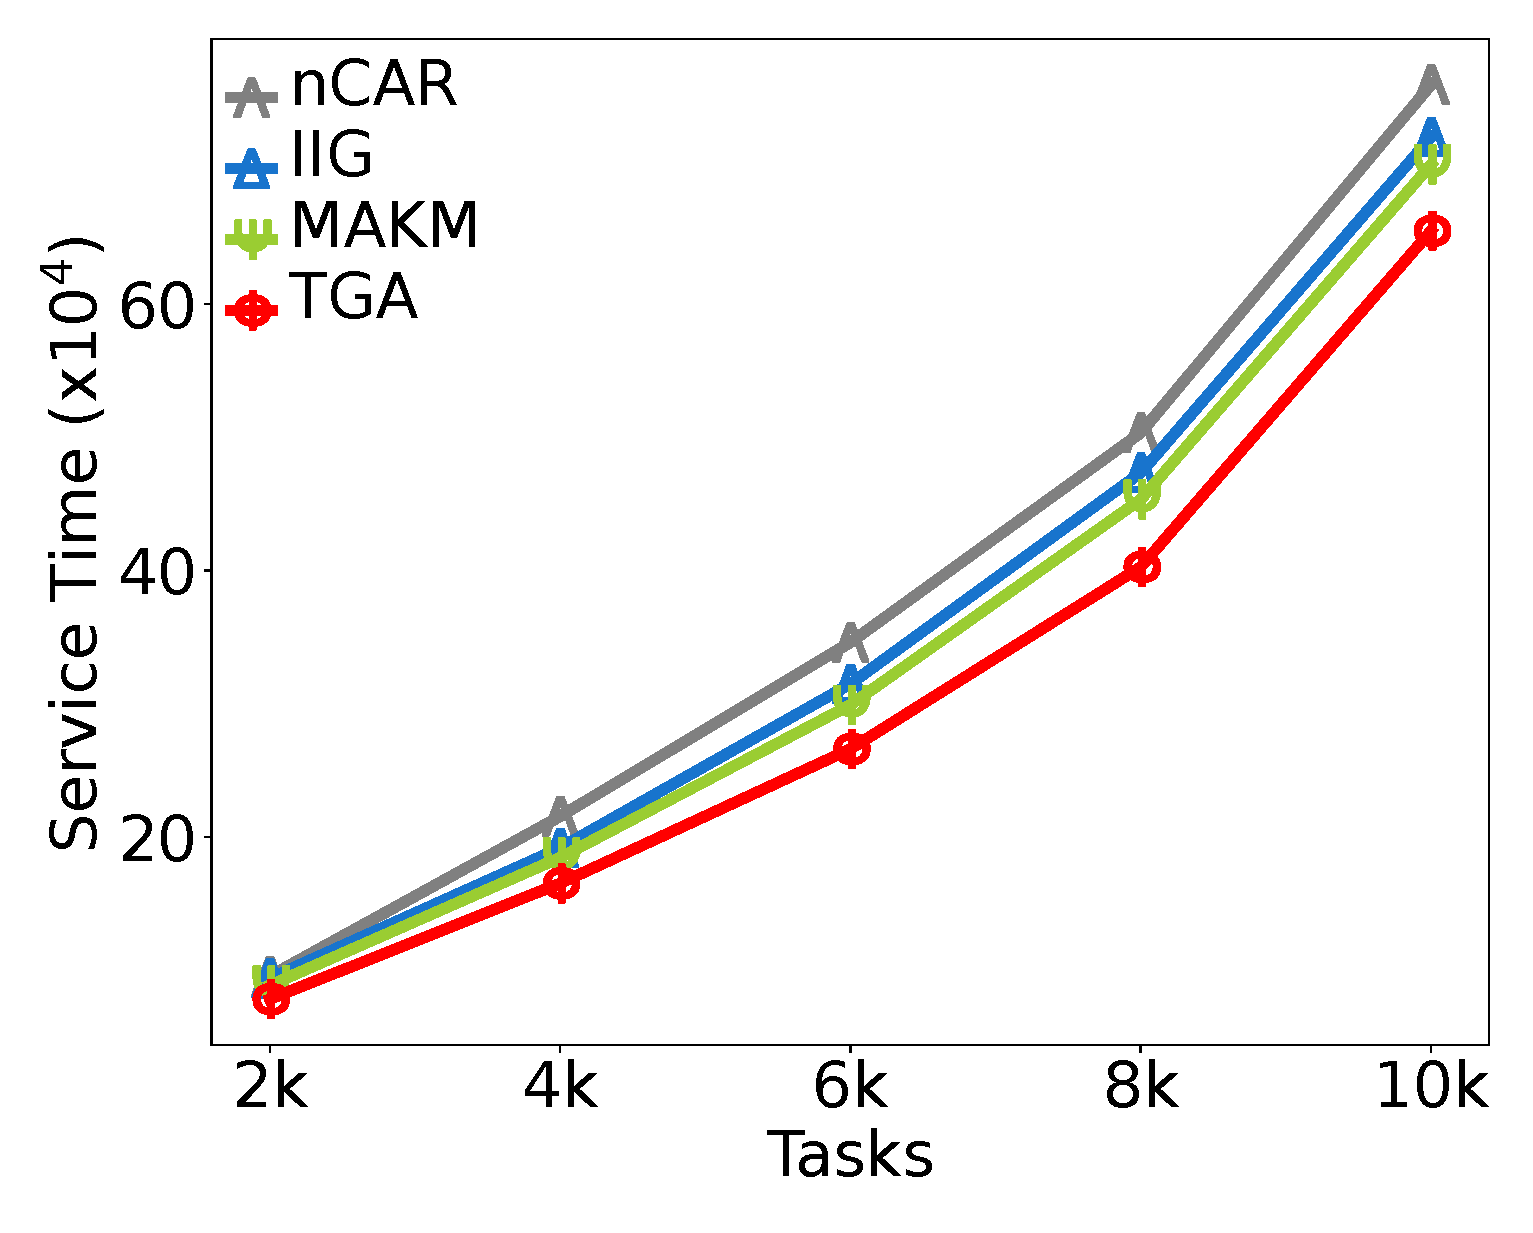
\includegraphics[width=0.3\linewidth]{Fig/taskNumST.eps}}
  \subfigure[$|A|$ vs. ST]{
    \label{fig:ep:taskMS}
    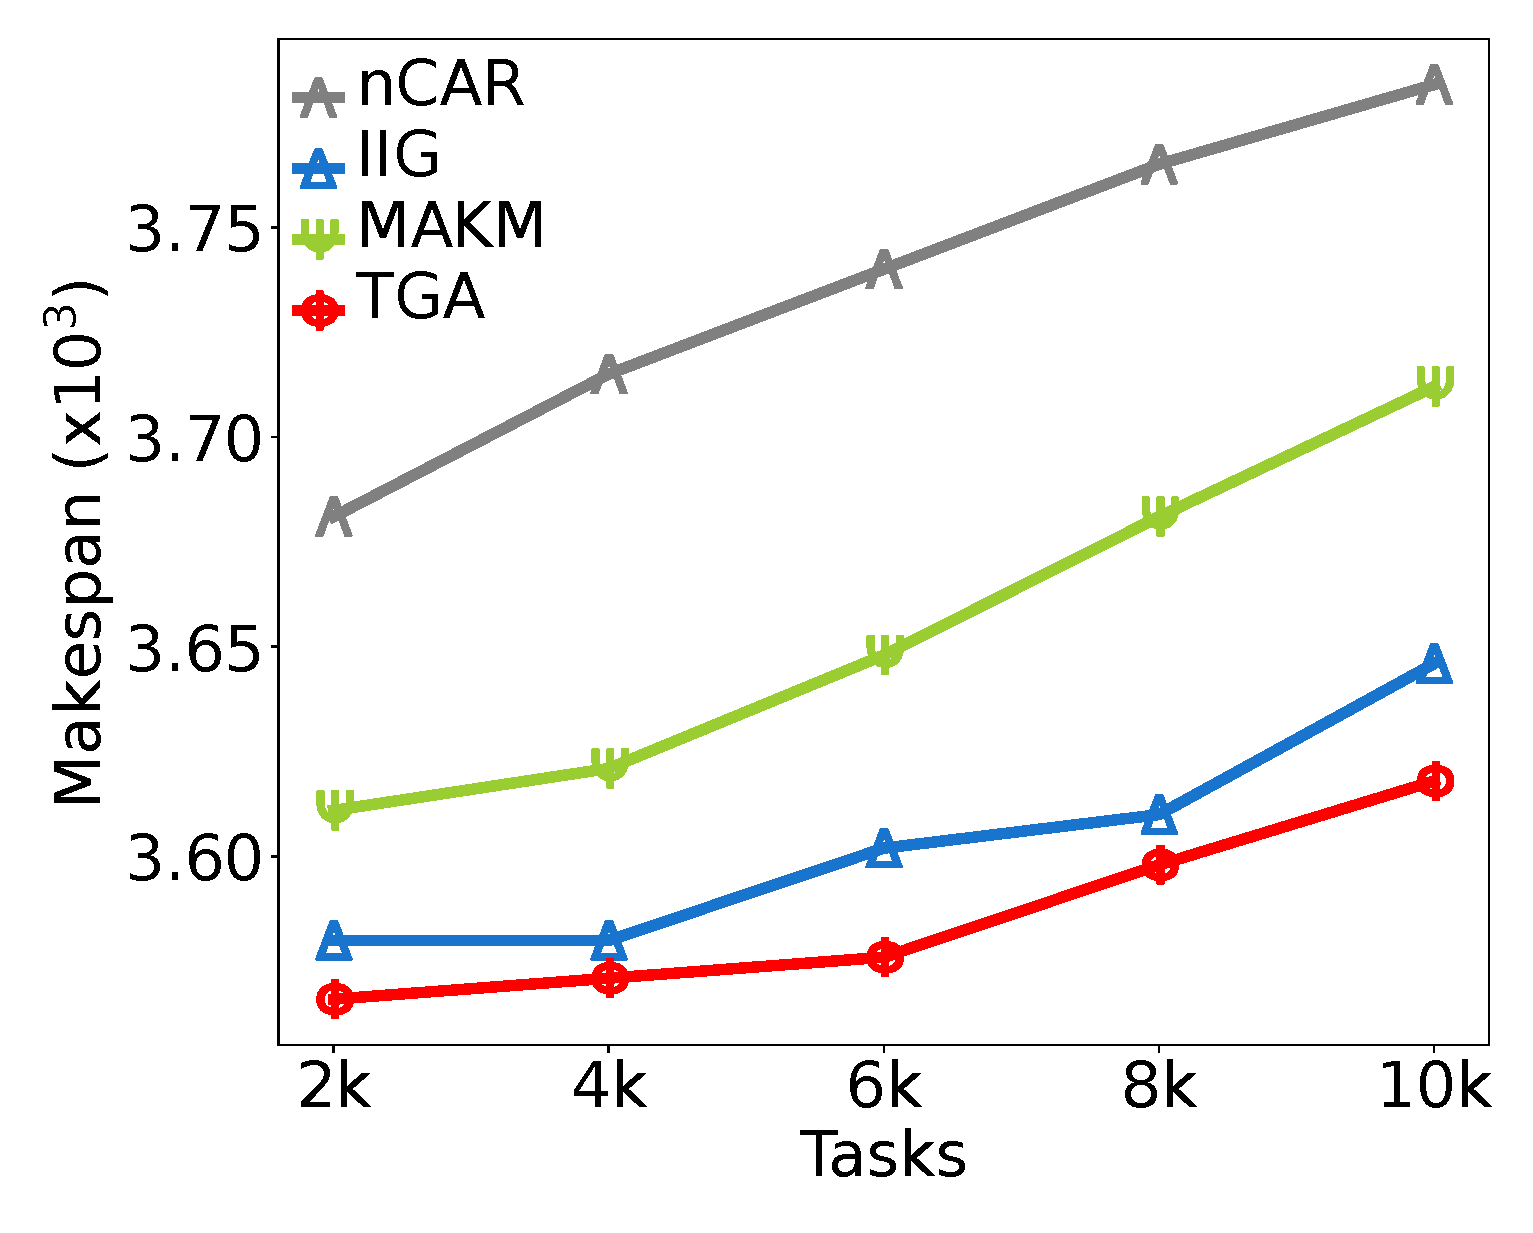
\includegraphics[width=0.3\linewidth]{Fig/taskNumMS.eps}}
  \subfigure[$c$ vs. ST]{
    \label{fig:ep:taskPT}
    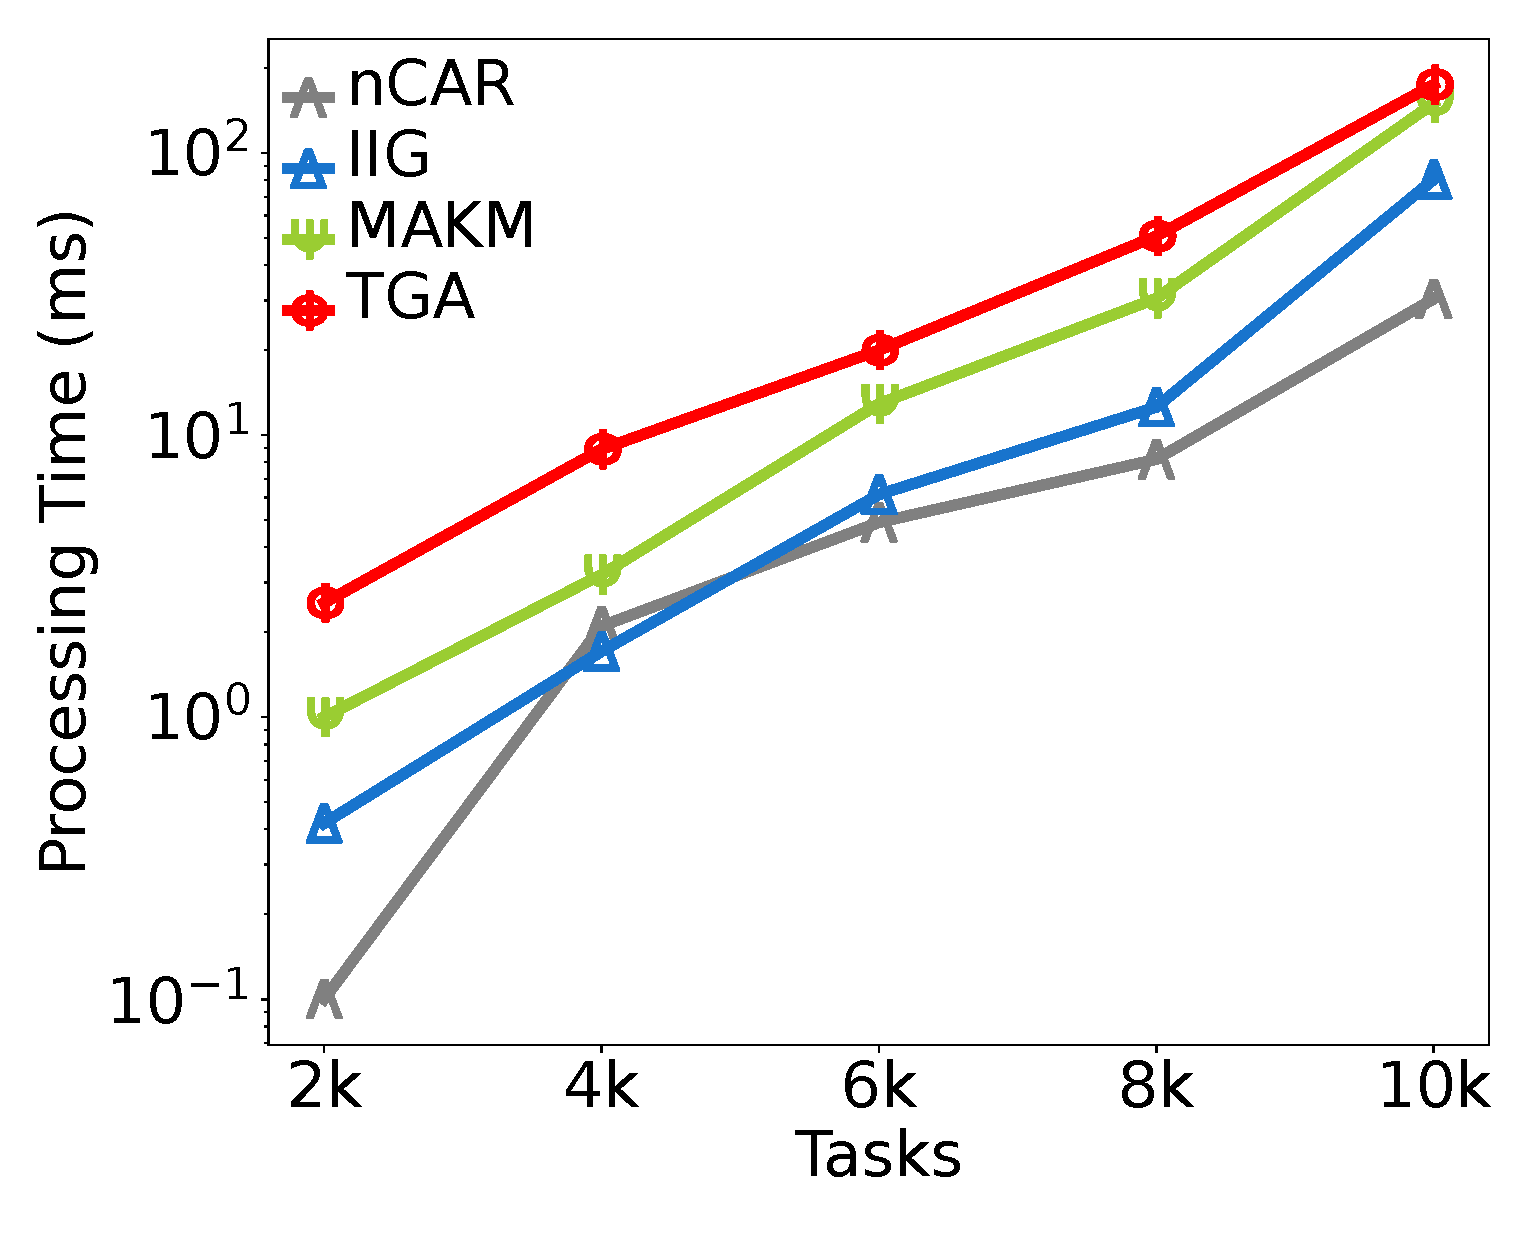
\includegraphics[width=0.3\linewidth]{Fig/taskNumPT.eps}}

  \subfigure[$|\Gamma|$ vs. MS]{
    \label{fig:ep:agentST}
    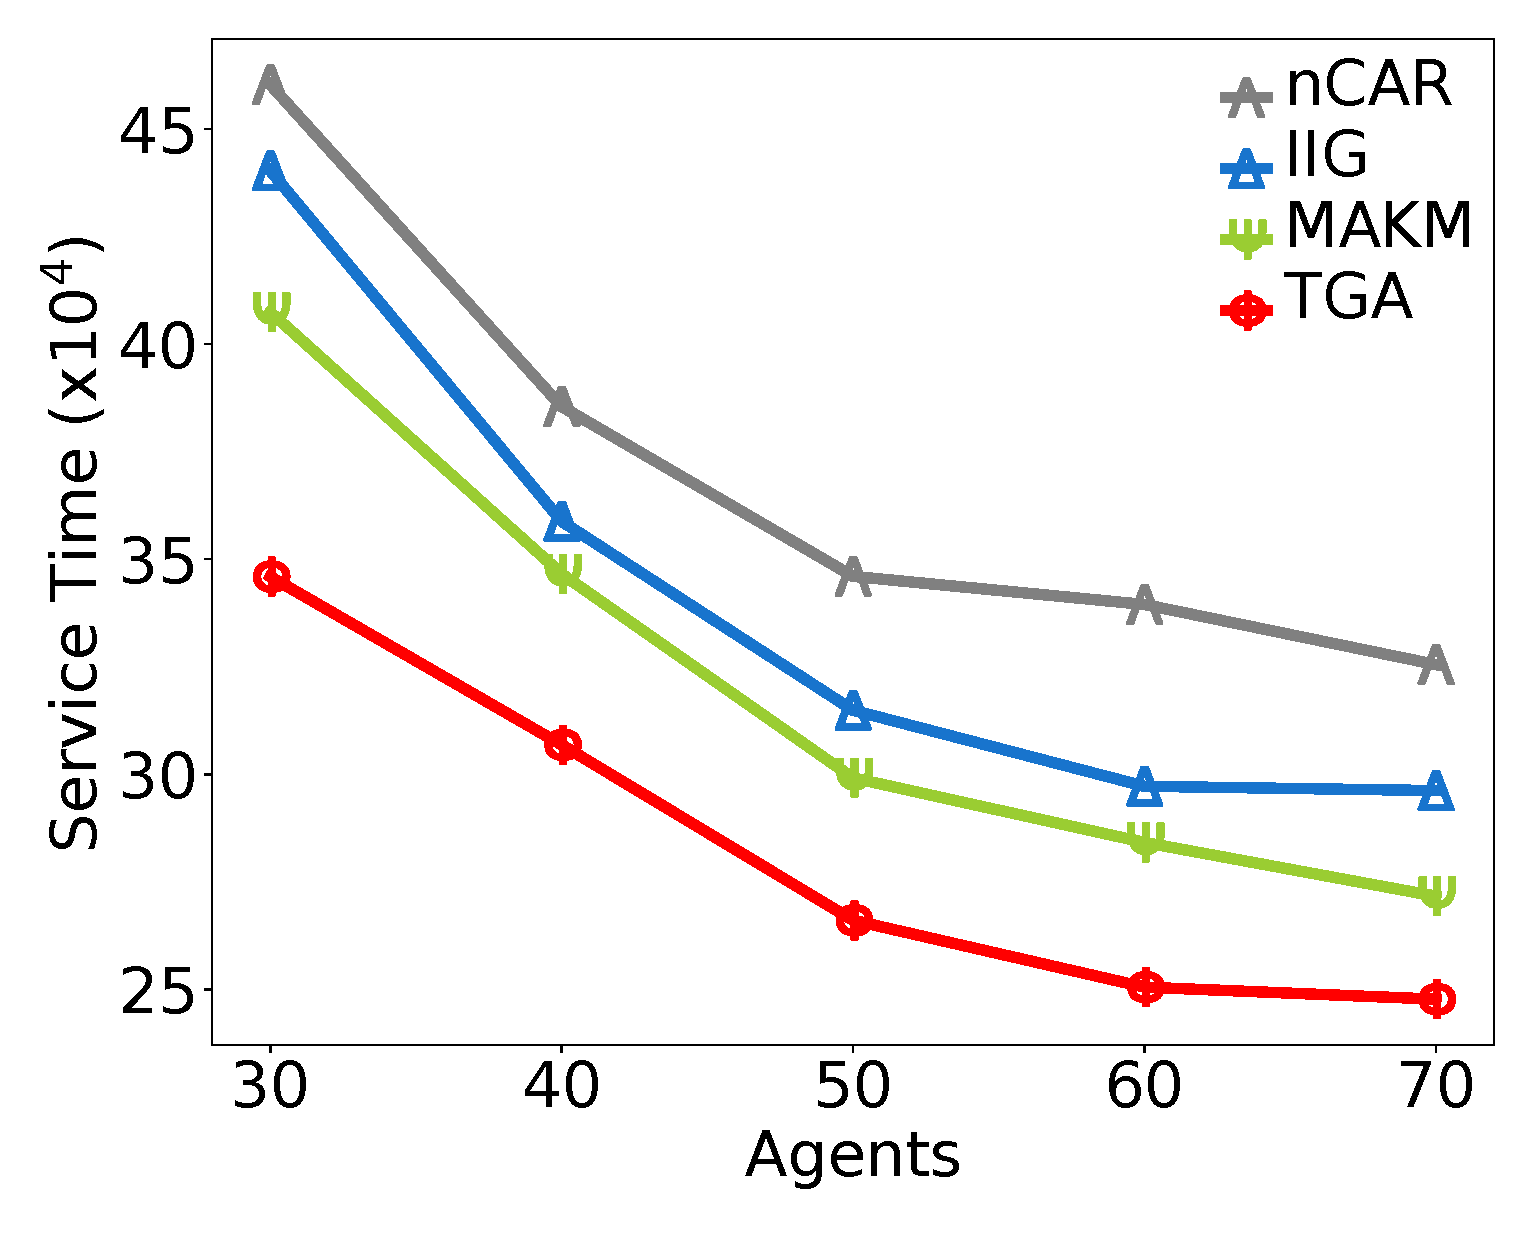
\includegraphics[width=0.3\linewidth]{Fig/agentNumST.eps}}
  \subfigure[$|A|$ vs. MS]{
    \label{fig:ep:agentMS}
    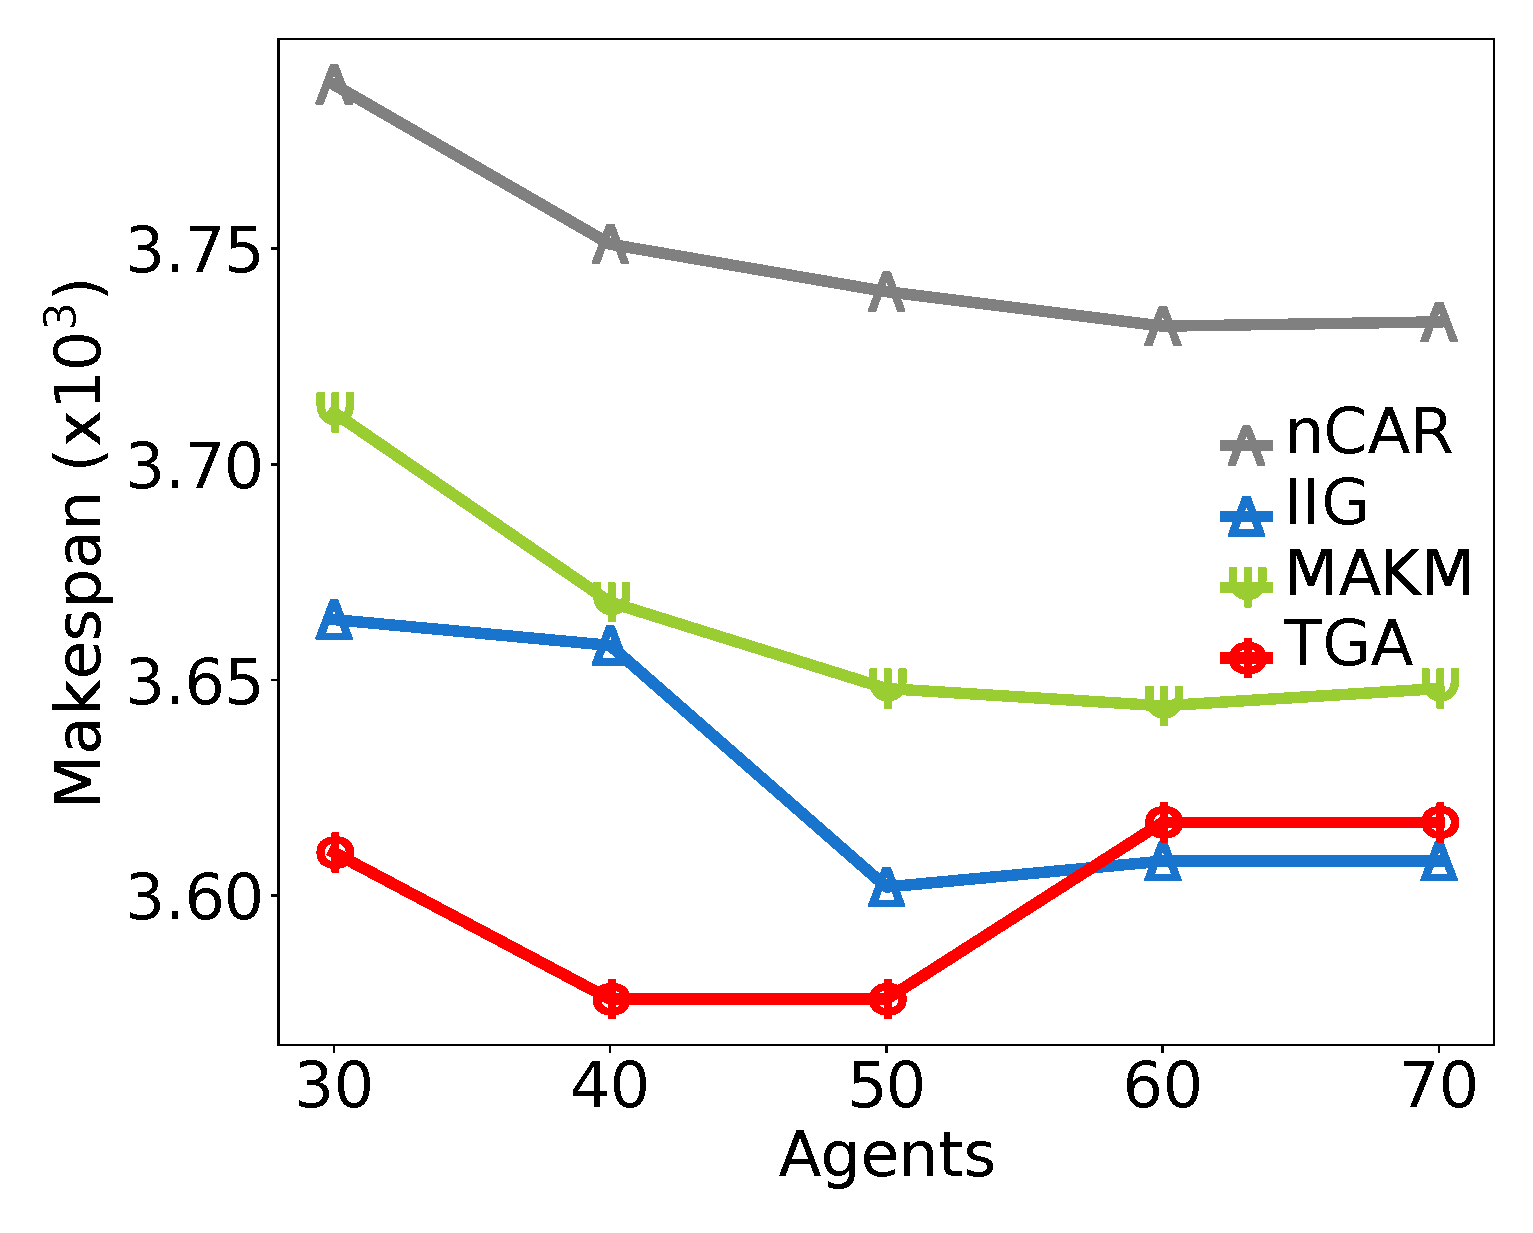
\includegraphics[width=0.3\linewidth]{Fig/agentNumMS.eps}}
  \subfigure[$c$ vs. MS]{
    \label{fig:ep:agentPT}
    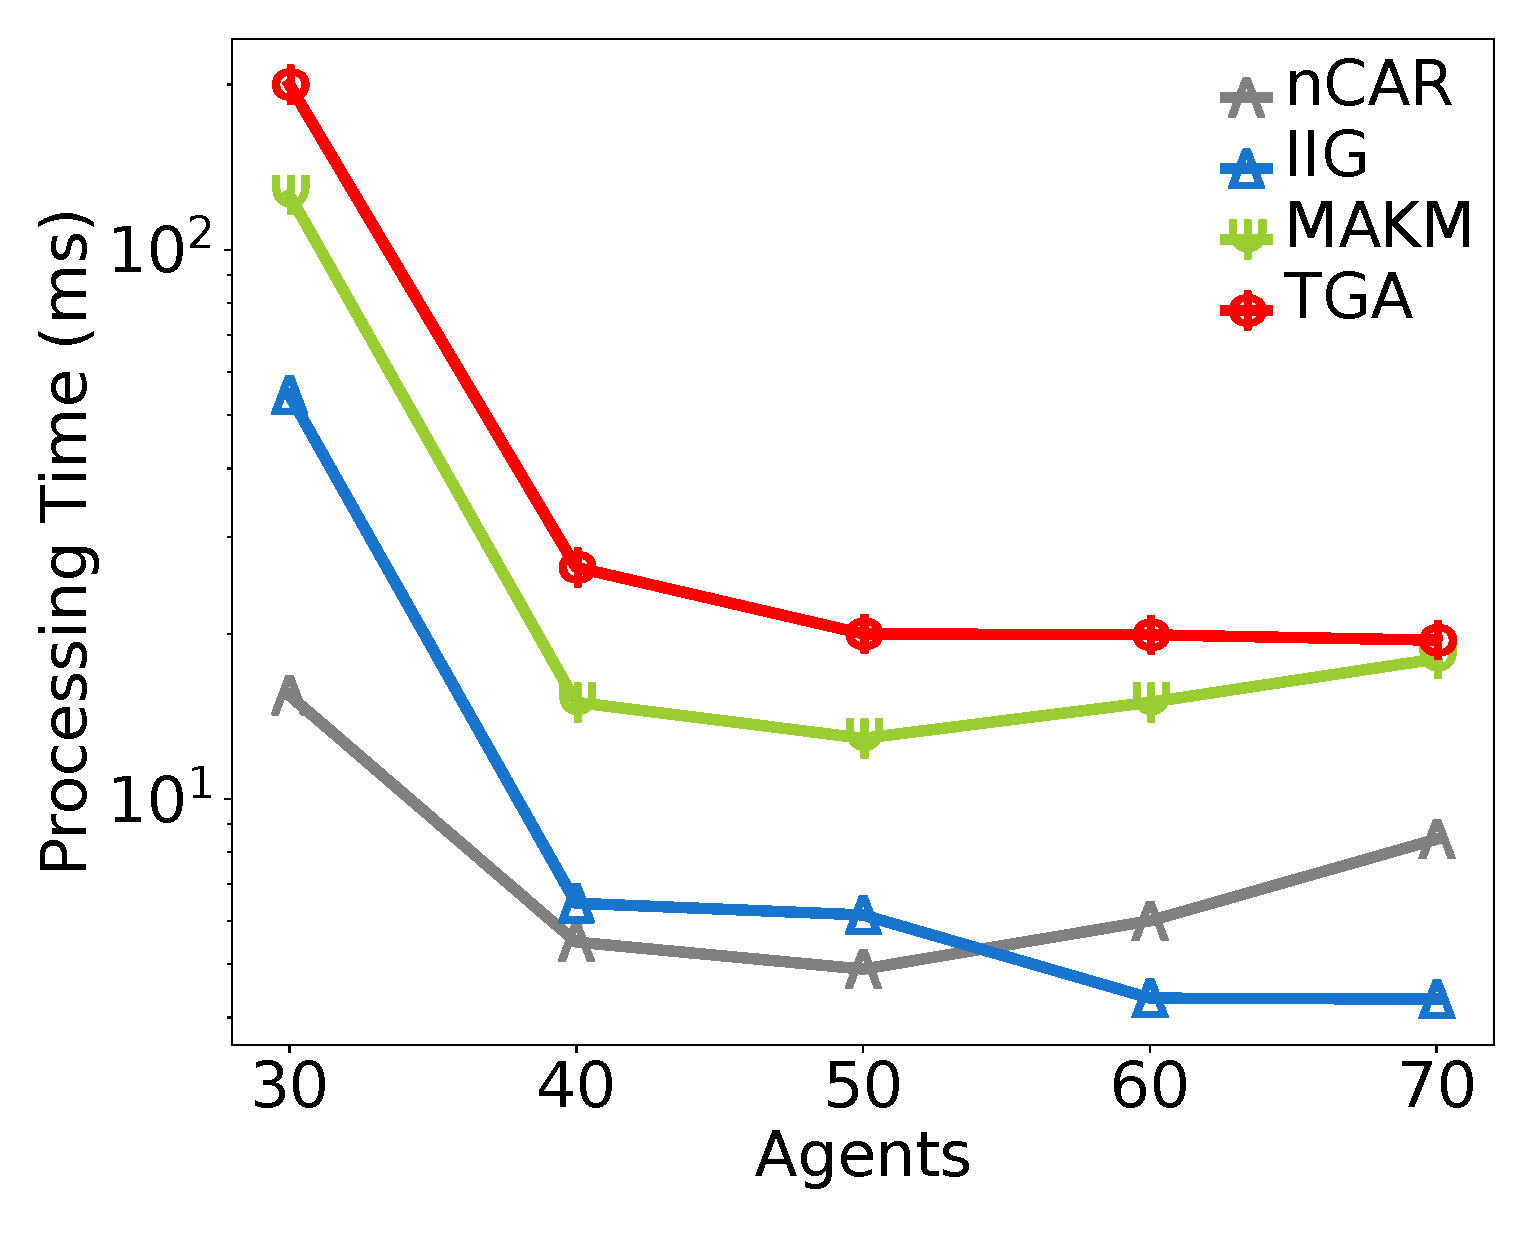
\includegraphics[width=0.3\linewidth]{Fig/agentNumPT.eps}}

  \subfigure[$|\Gamma|$ vs. PT]{
    \label{fig:ep:capacityST}
    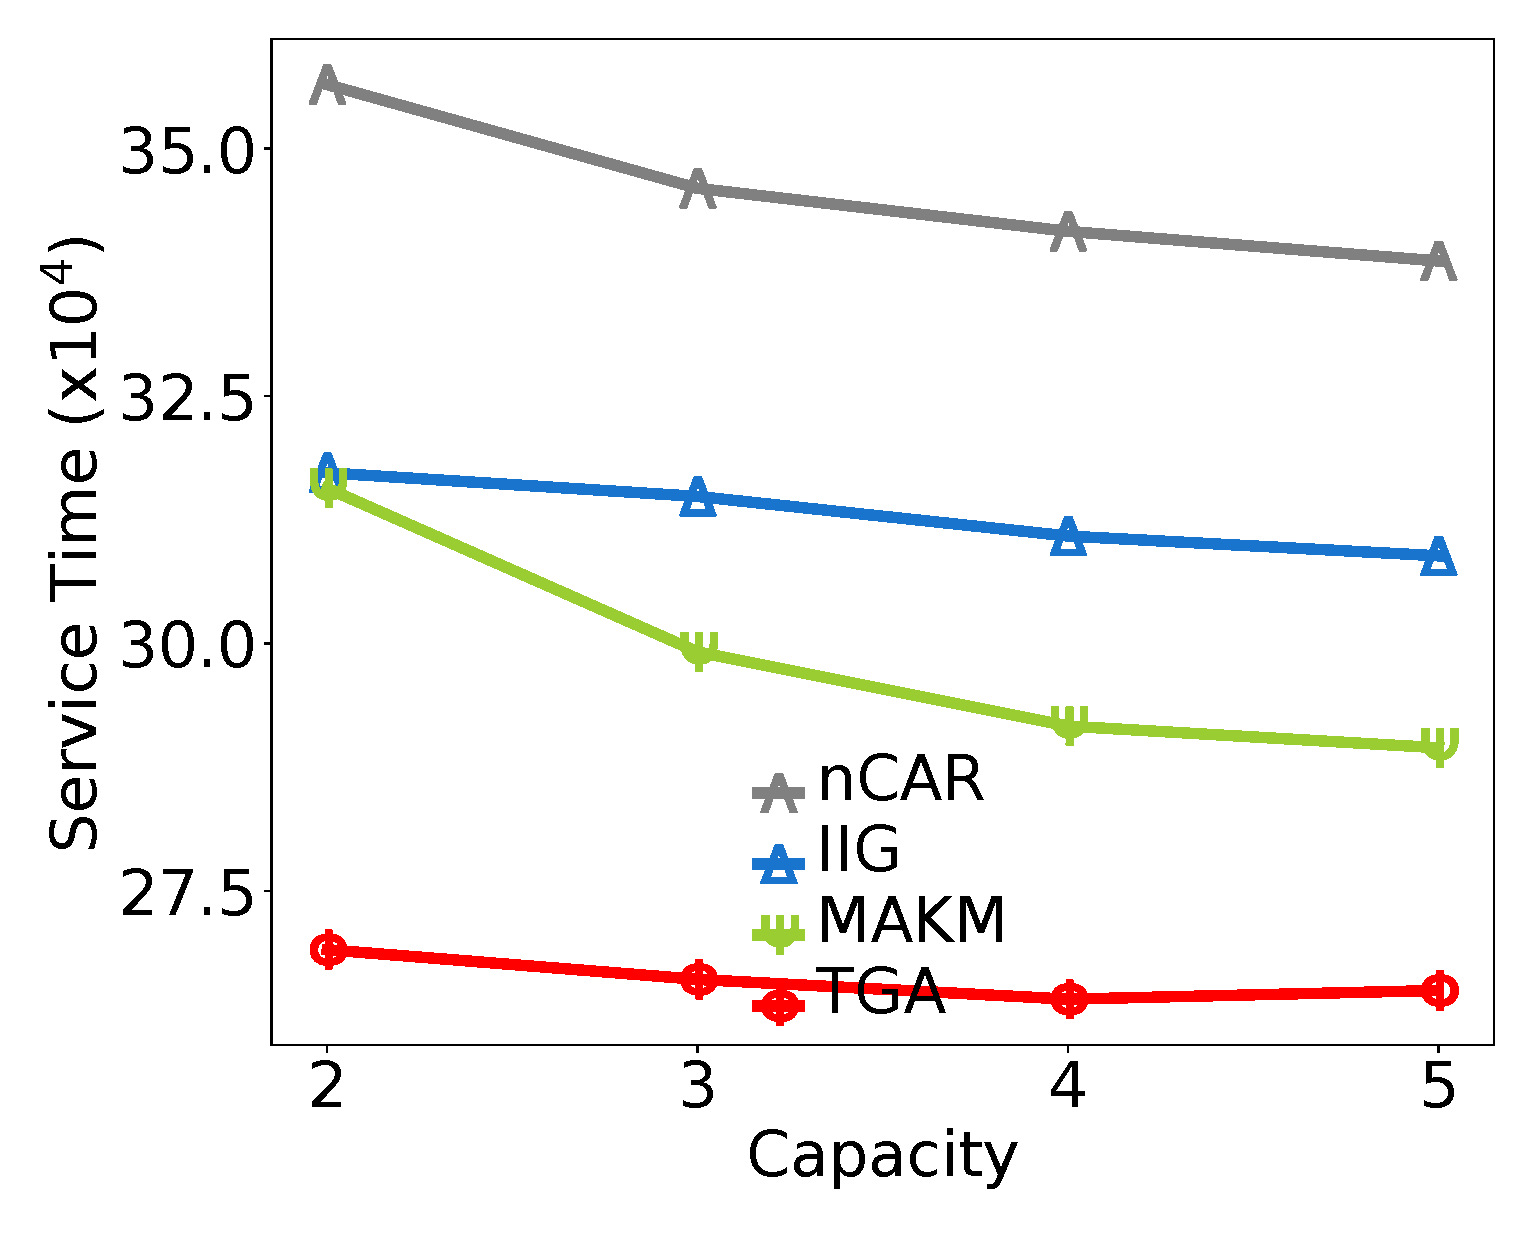
\includegraphics[width=0.3\linewidth]{Fig/capacityST.eps}}
  \subfigure[$|A|$ vs. PT]{
    \label{fig:ep:capacityMS}
    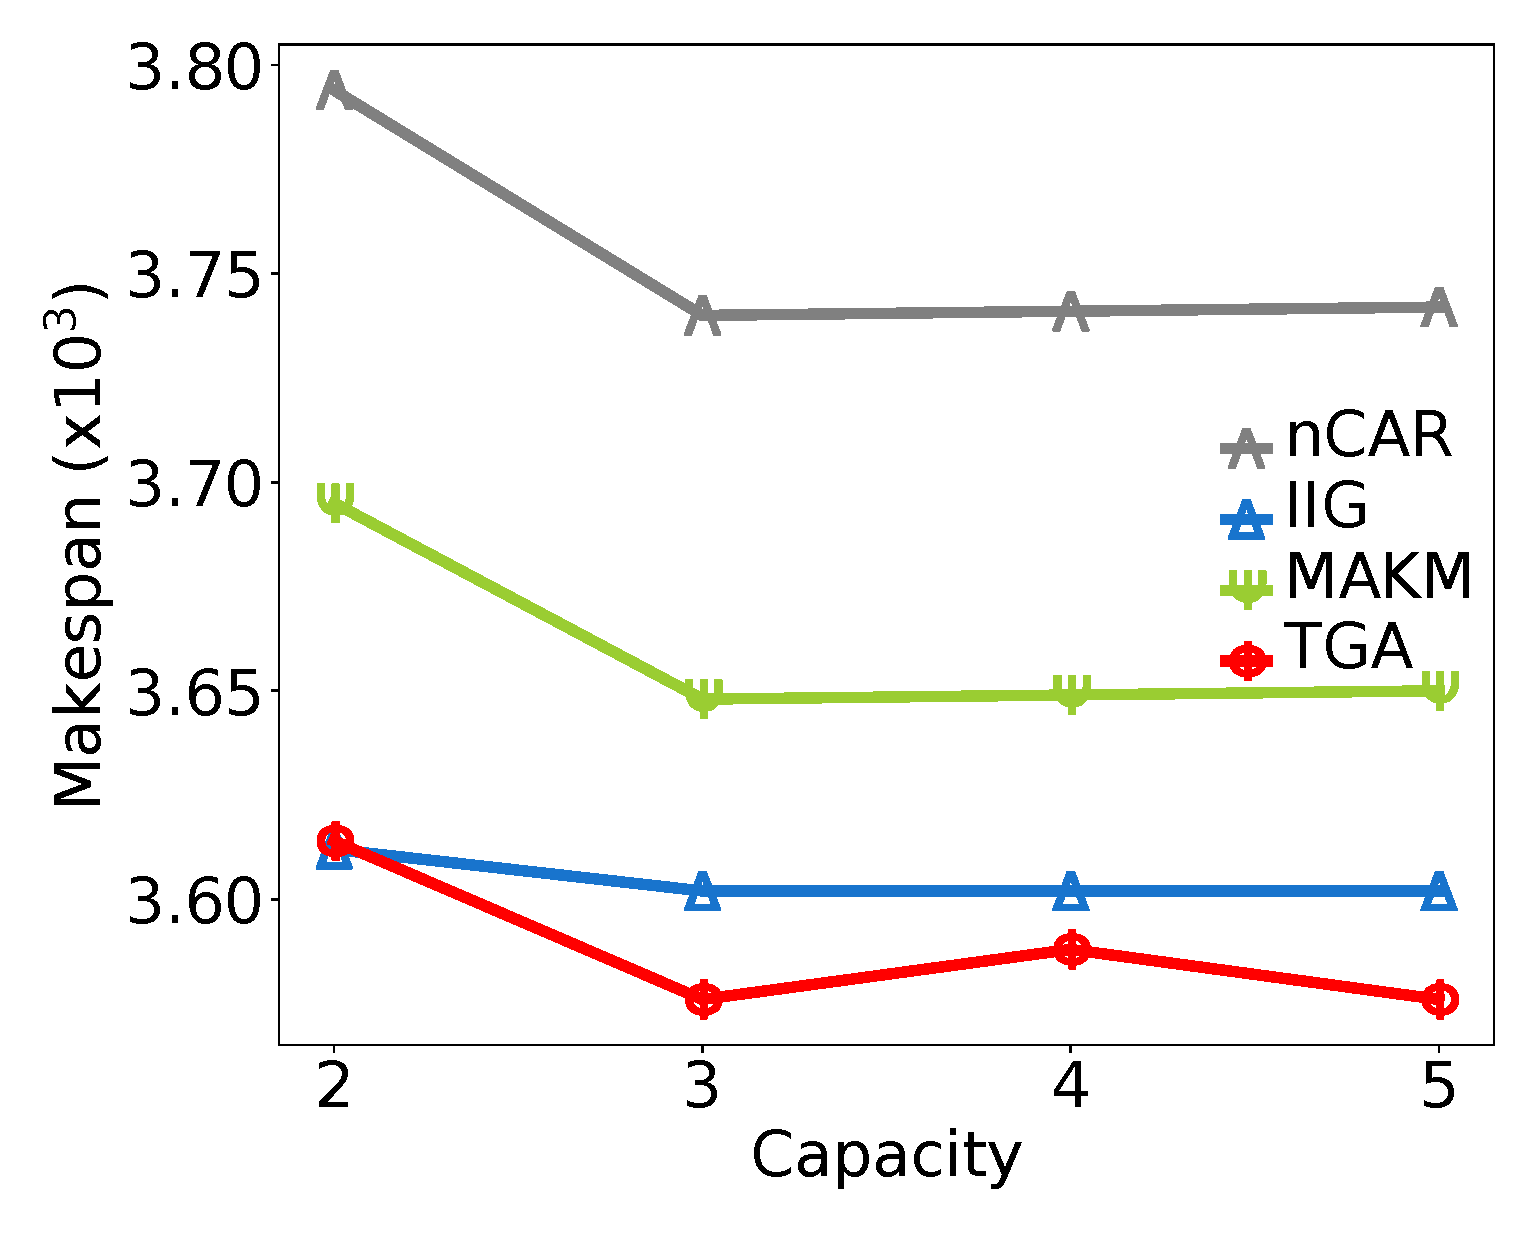
\includegraphics[width=0.3\linewidth]{Fig/capacityMS.eps}}
  \subfigure[$c$ vs. PT]{
    \label{fig:ep:capacityPT}
    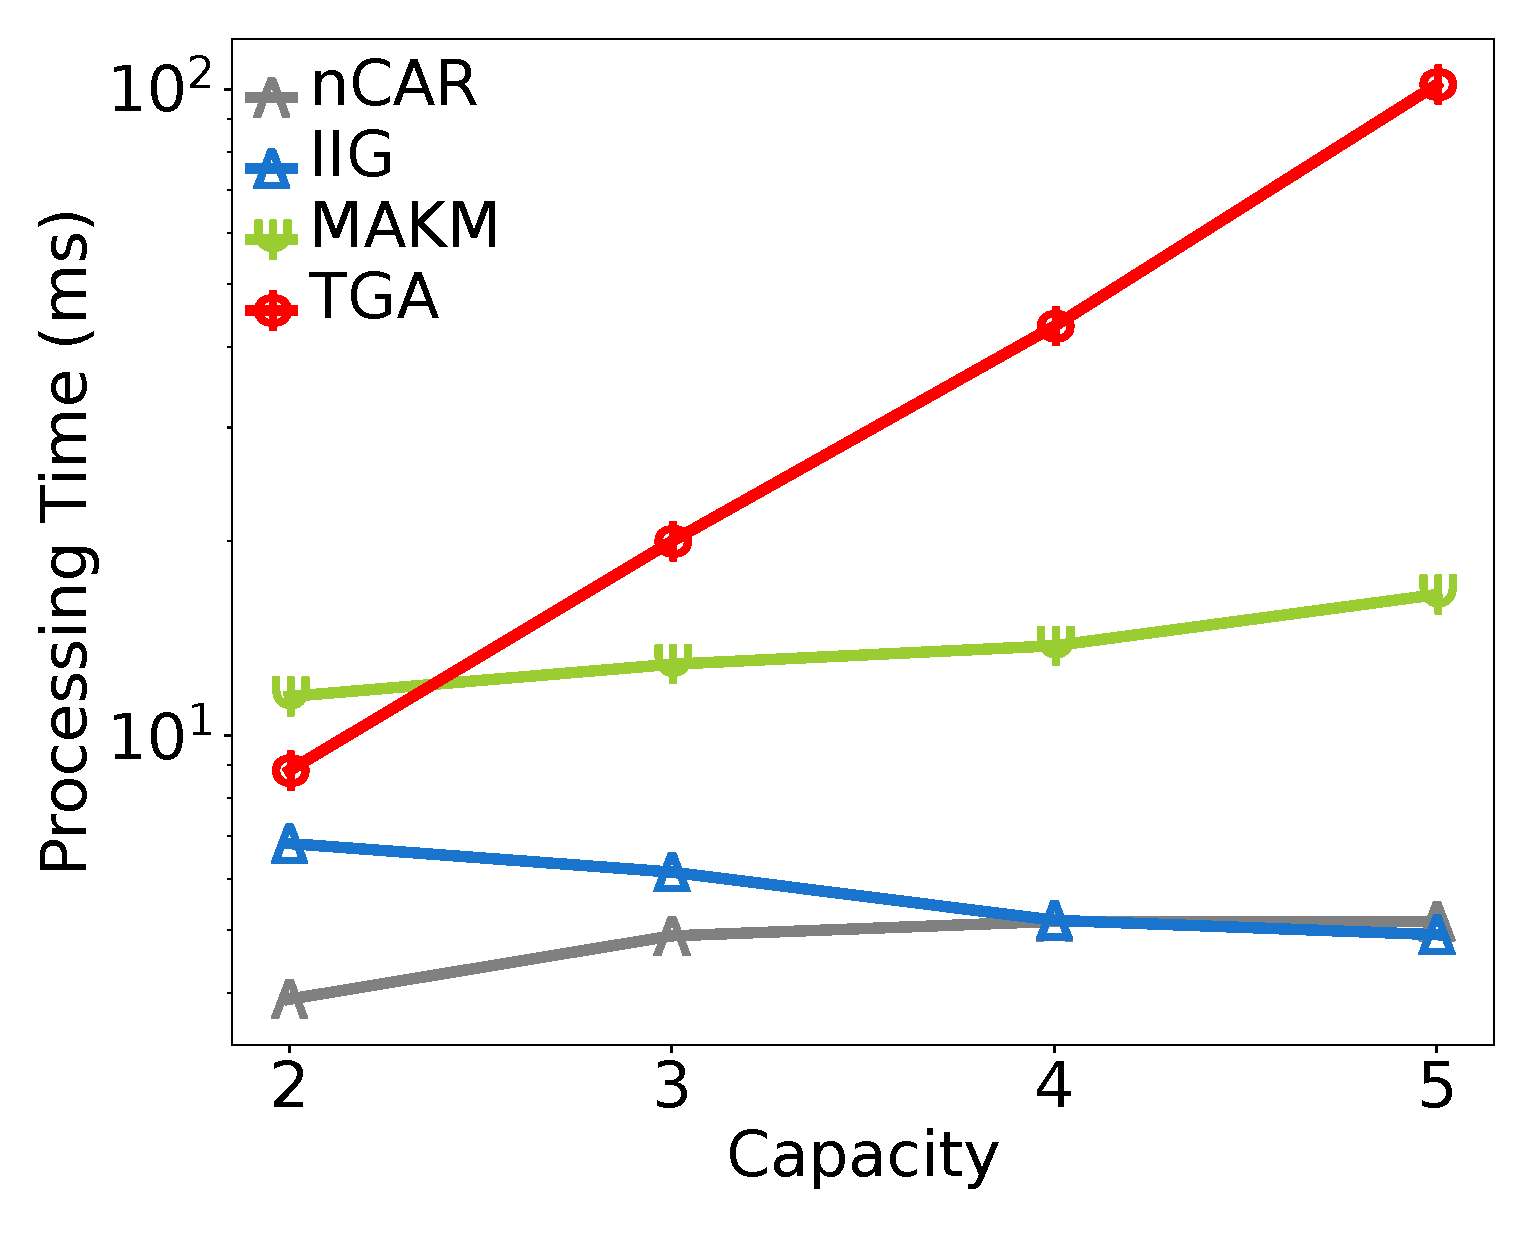
\includegraphics[width=0.3\linewidth]{Fig/capacityPT.eps}}

  \caption{Performance of $|\Gamma|$ \textbf{vs. ST, MS and PT}}
  \label{fig:ep:task}
  \Description{Performance of $|\Gamma|$ \textbf{vs. ST, MS and PT}}
\end{figure*}

The experimental settings are shown in Table~\ref{tab:settings}.
We vary the number of tasks from 2k to 10k,
the number of agents from 30 to 70,
and the max capacity of agents from 2 to 6.
The bold values are the default settings.
The evaluation metrics include service time ($ST$), makespan ($MS$), and processing time ($PT$).
Finally, we compare the proposed algorithm with the following algorithms:
\begin{itemize}
  \item nCAR algorithm~\cite{sarkar2018scalable},
  which clusters tasks based on the nearest neighbor,
  and constructs a route for each cluster by mapping it to a TSP.
  \item IIG algorithm~\cite{zhang2022effective},
  which generates an initial solution by a greedy strategy,
  and iteratively improves the solution by a local search strategy.
  \item Multi-angle K-means algorithm~\cite{electronics12183842},
  which uses the multi-angle K-means algorithm to divide the set of tasks into groups,
  and uses GA algorithm to perform path planning.
  \item TGA algorithm, which uses KCHC Algorithm to divide the set of tasks into groups,
  and allocates task groups to agents.
\end{itemize}


\subsection{Experimental Results}

\textbf{Performance of task number $|\Gamma|$:} As shown in Figure~\ref{fig:ep:taskST},
~\ref{fig:ep:taskMS} and ~\ref{fig:ep:taskPT},
we can see the impact of the number of tasks on $ST$, $MS$ and $PT$.
When the number of tasks increases,
the $ST$, $MS$ and $PT$ increase,
since the agents need more time to complete more tasks, in each batch.
The proposed TGA algorithm outperforms the other algorithms on $ST$ and $MS$,
since it can allocate task groups to agents more efficiently.
As shown in Figure~\ref{fig:ep:taskST},
when the number of tasks is 6k,
TGA algorithm reduces $ST$ by 20.6\% compared with nCAR algorithm,
and by 15.2\% compared with IIG algorithm.
 
\textbf{Performance of agent number $|A|$:}
figure~\ref{fig:ep:agentST}, ~\ref{fig:ep:agentMS} and ~\ref{fig:ep:agentPT}
illustrate the impact of the number of agents on $ST$, $MS$ and $PT$.
When the number of agents increases,
the $ST$ is reduced, and the trend is gradually decreasing.
Because, starting with a small number of agents, 
the waiting time for the task is extended, 
but as the number of agents increases and approaches full saturation, 
the decreasing trend of ST slowly reduces.
In Figure~\ref{fig:ep:agentMS},
$MS$ has a similar trend to $ST$, even slightly higher.
Although TGA algorithm has a higher $PT$ than other algorithms,
it has a lower $ST$ and $MS$.

\textbf{Performance of capacity $c$:}
The impact of the max capacity of agents on $ST$, $MS$ and $PT$ is shown 
in Figure~\ref{fig:ep:capacityST}, ~\ref{fig:ep:capacityMS} and ~\ref{fig:ep:capacityPT}.
A higher capacity of agents can lead to a lower $ST$ and $MS$.
As the capacity of agents increases, the $ST$ and $MS$ decrease.
The increase in the capacity of agents means
that the agents can carry more tasks simultaneously,
which leads that all algorithms have better performance on $ST$ and $MS$.
Sepcially, all algorithms have a similar performance on $PT$,
since the capacity of agents does not affect the processing time of tasks.
Howerver, $PT$ of the TGA algorithm has obviously increased by capacity,
since the more capacity, the more complexity of the task group allocation.


% \begin{figure*}
%   \centering
%   \subfigure[$|\Gamma|$ vs. MS]{
%     \label{fig:ep:agentST}
%     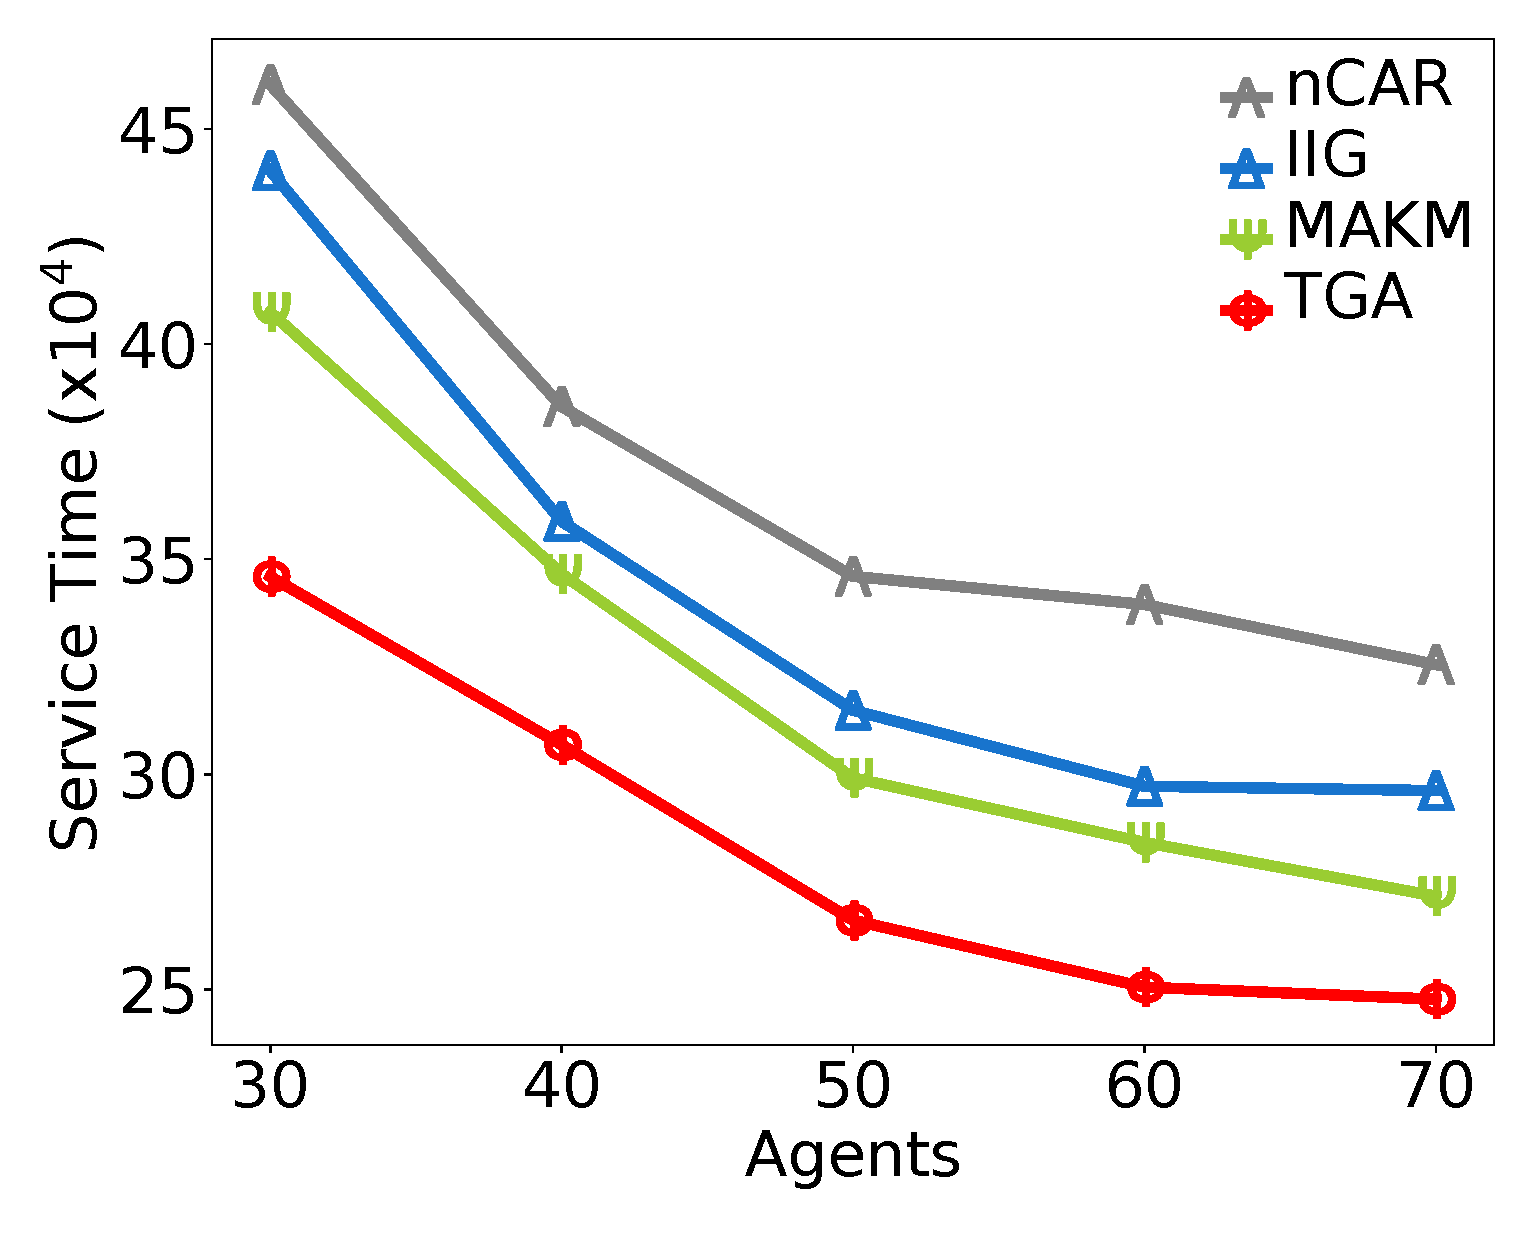
\includegraphics[width=0.3\linewidth]{Fig/agentNumST.eps}}
%   \subfigure[$|A|$ vs. MS]{
%     \label{fig:ep:agentMS}
%     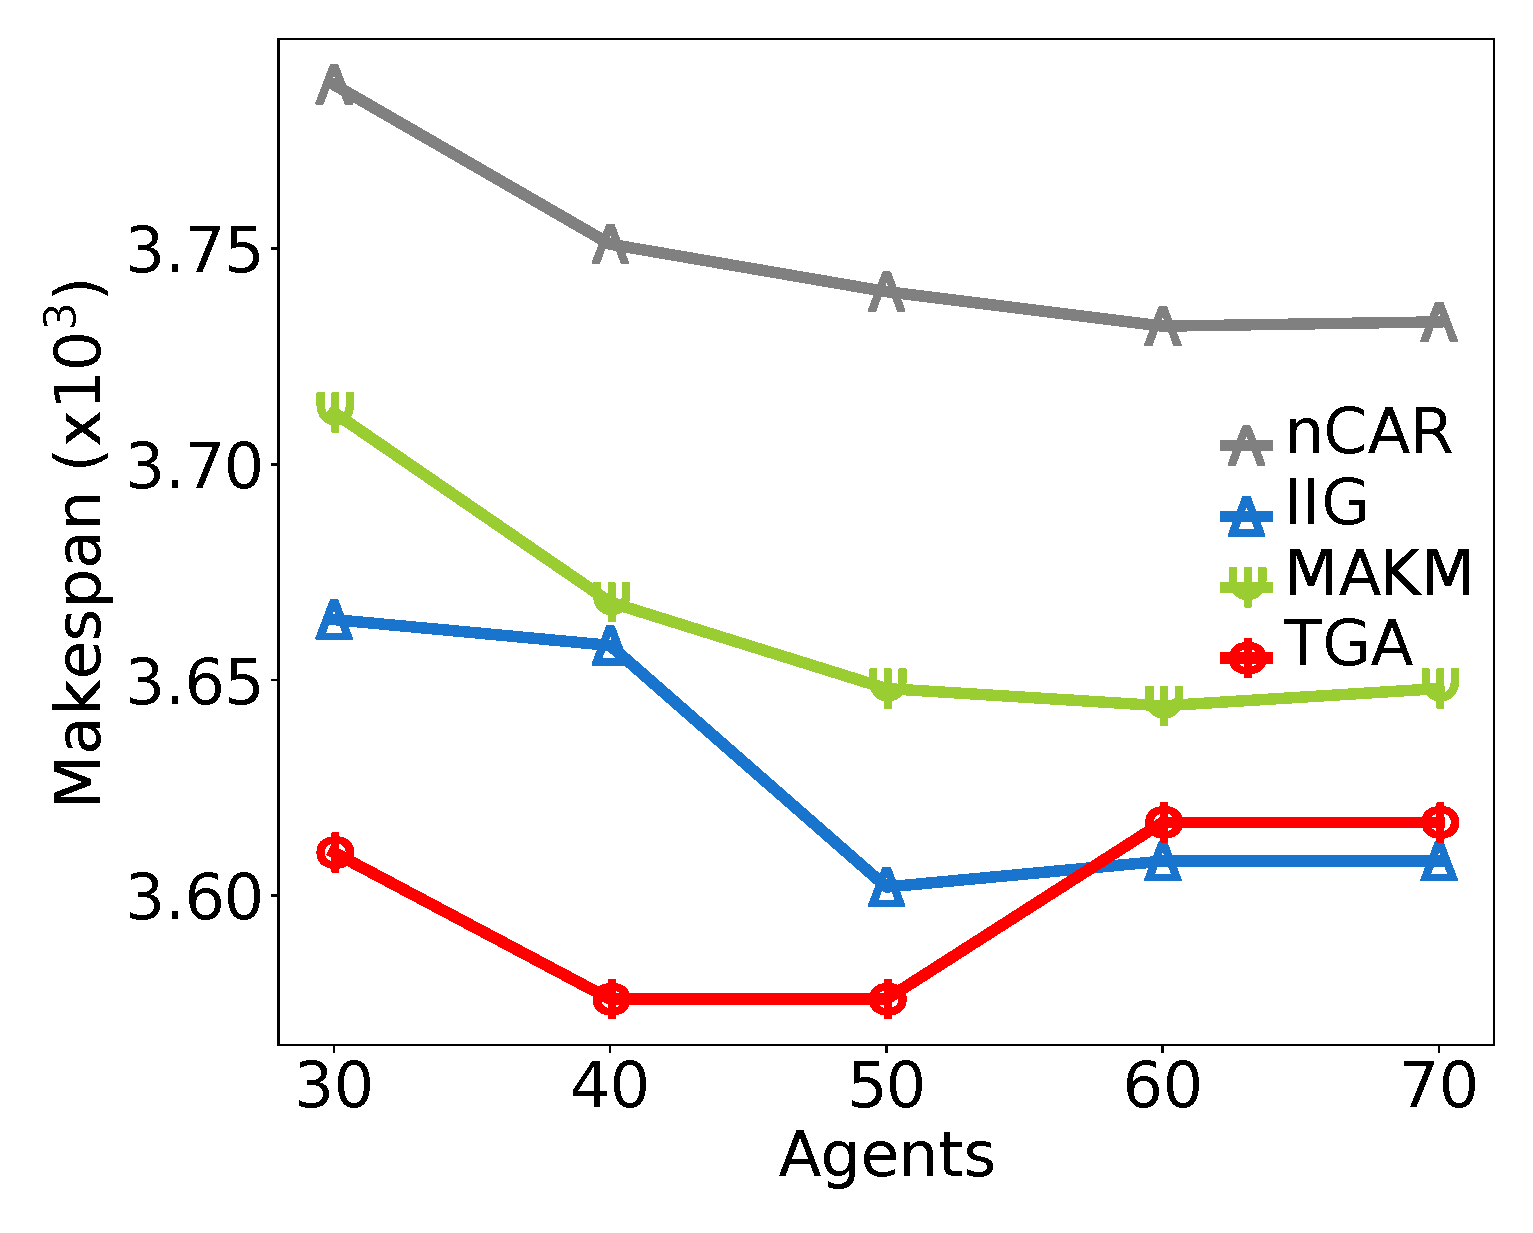
\includegraphics[width=0.3\linewidth]{Fig/agentNumMS.eps}}
%   \subfigure[$c$ vs. MS]{
%     \label{fig:ep:agentPT}
%     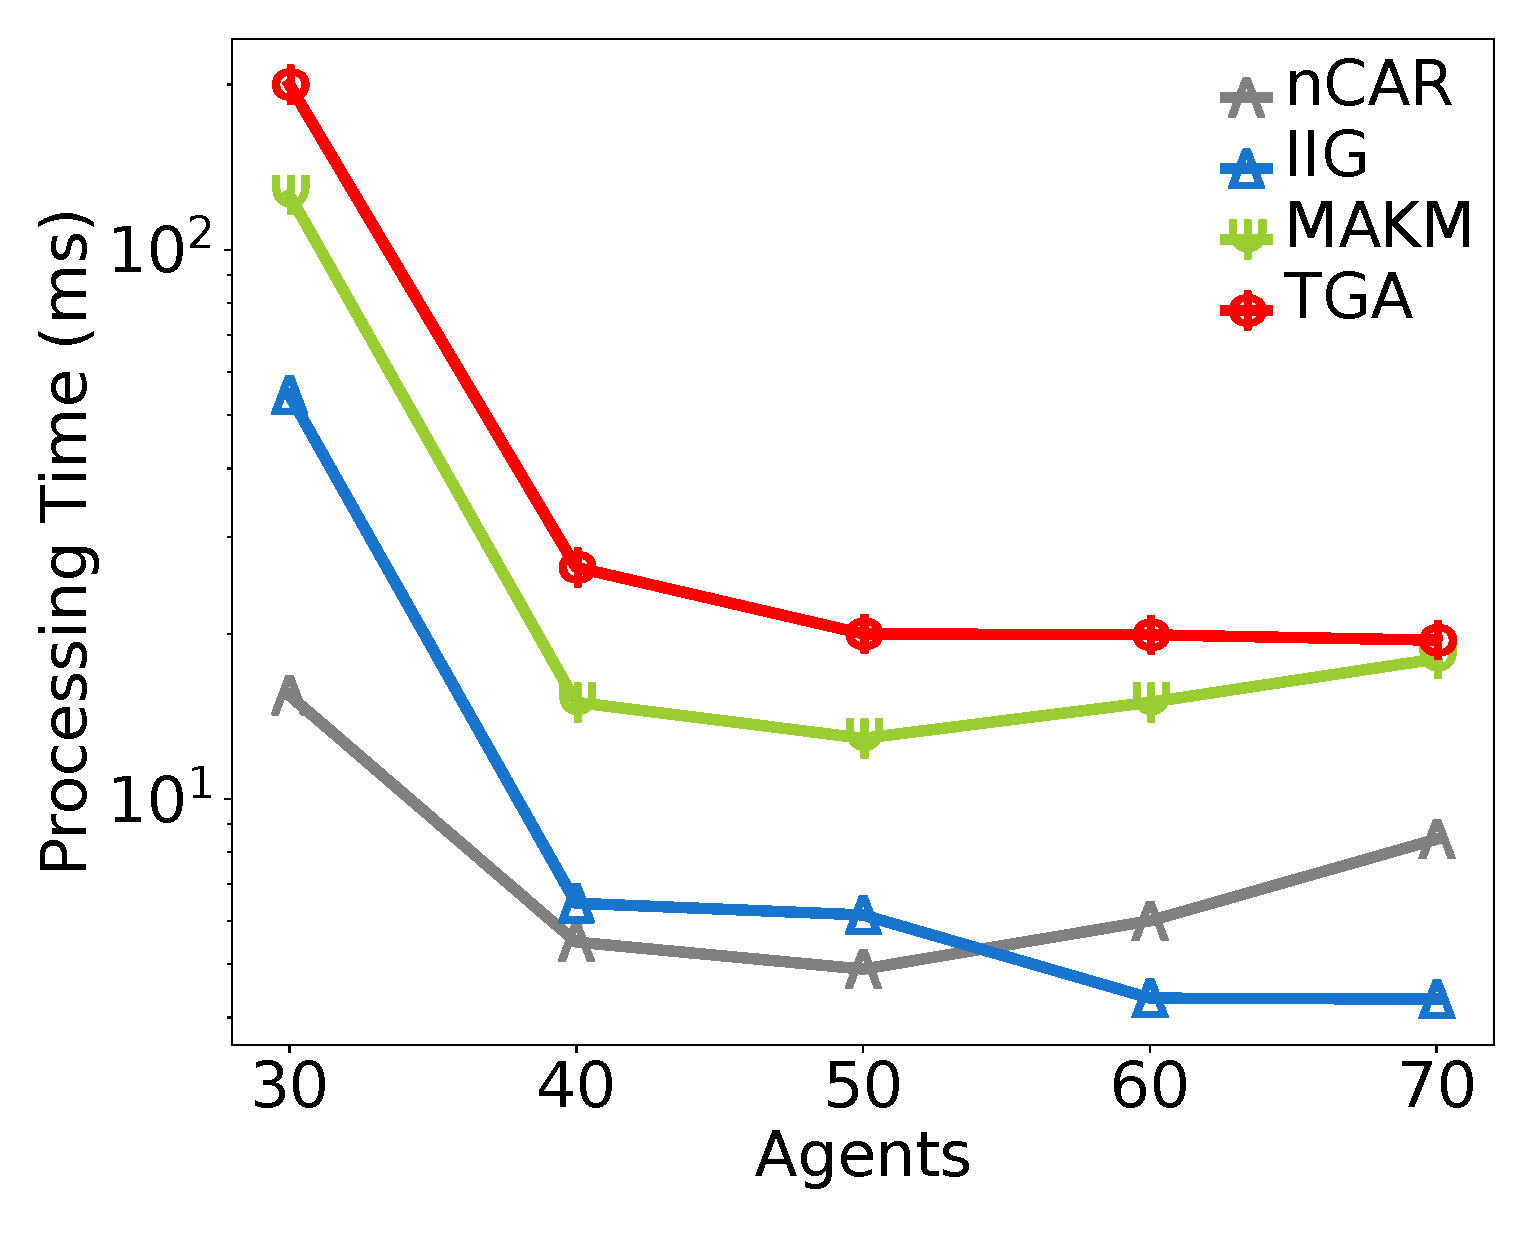
\includegraphics[width=0.3\linewidth]{Fig/agentNumPT.eps}}
%   \caption{Performance of $|A|$ \textbf{vs. ST, MS and PT}}
%   \label{fig:ep:agent}
%   \Description{Performance of $|A|$ \textbf{vs. ST, MS and PT}}
% \end{figure*}



% \begin{figure*}
%   \centering
%   \subfigure[$|\Gamma|$ vs. PT]{
%     \label{fig:ep:capacityST}
%     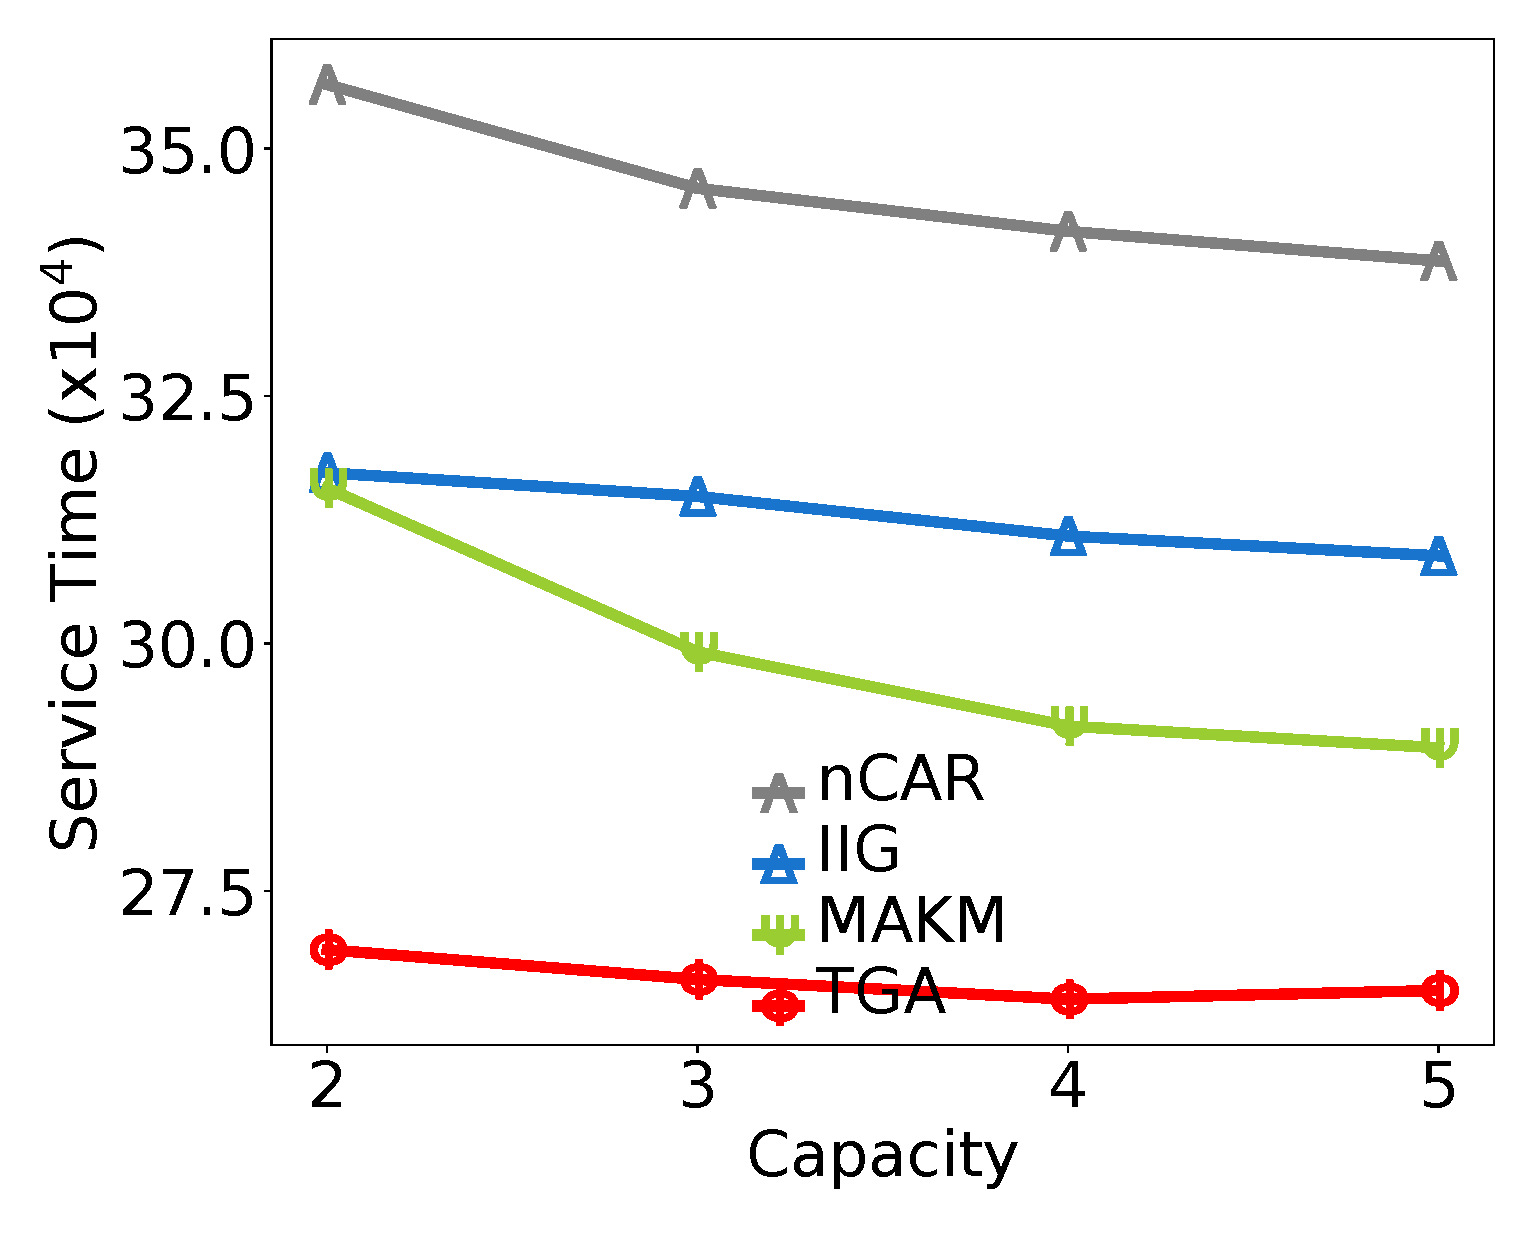
\includegraphics[width=0.3\linewidth]{Fig/capacityST.eps}}
%   \subfigure[$|A|$ vs. PT]{
%     \label{fig:ep:capacityMS}
%     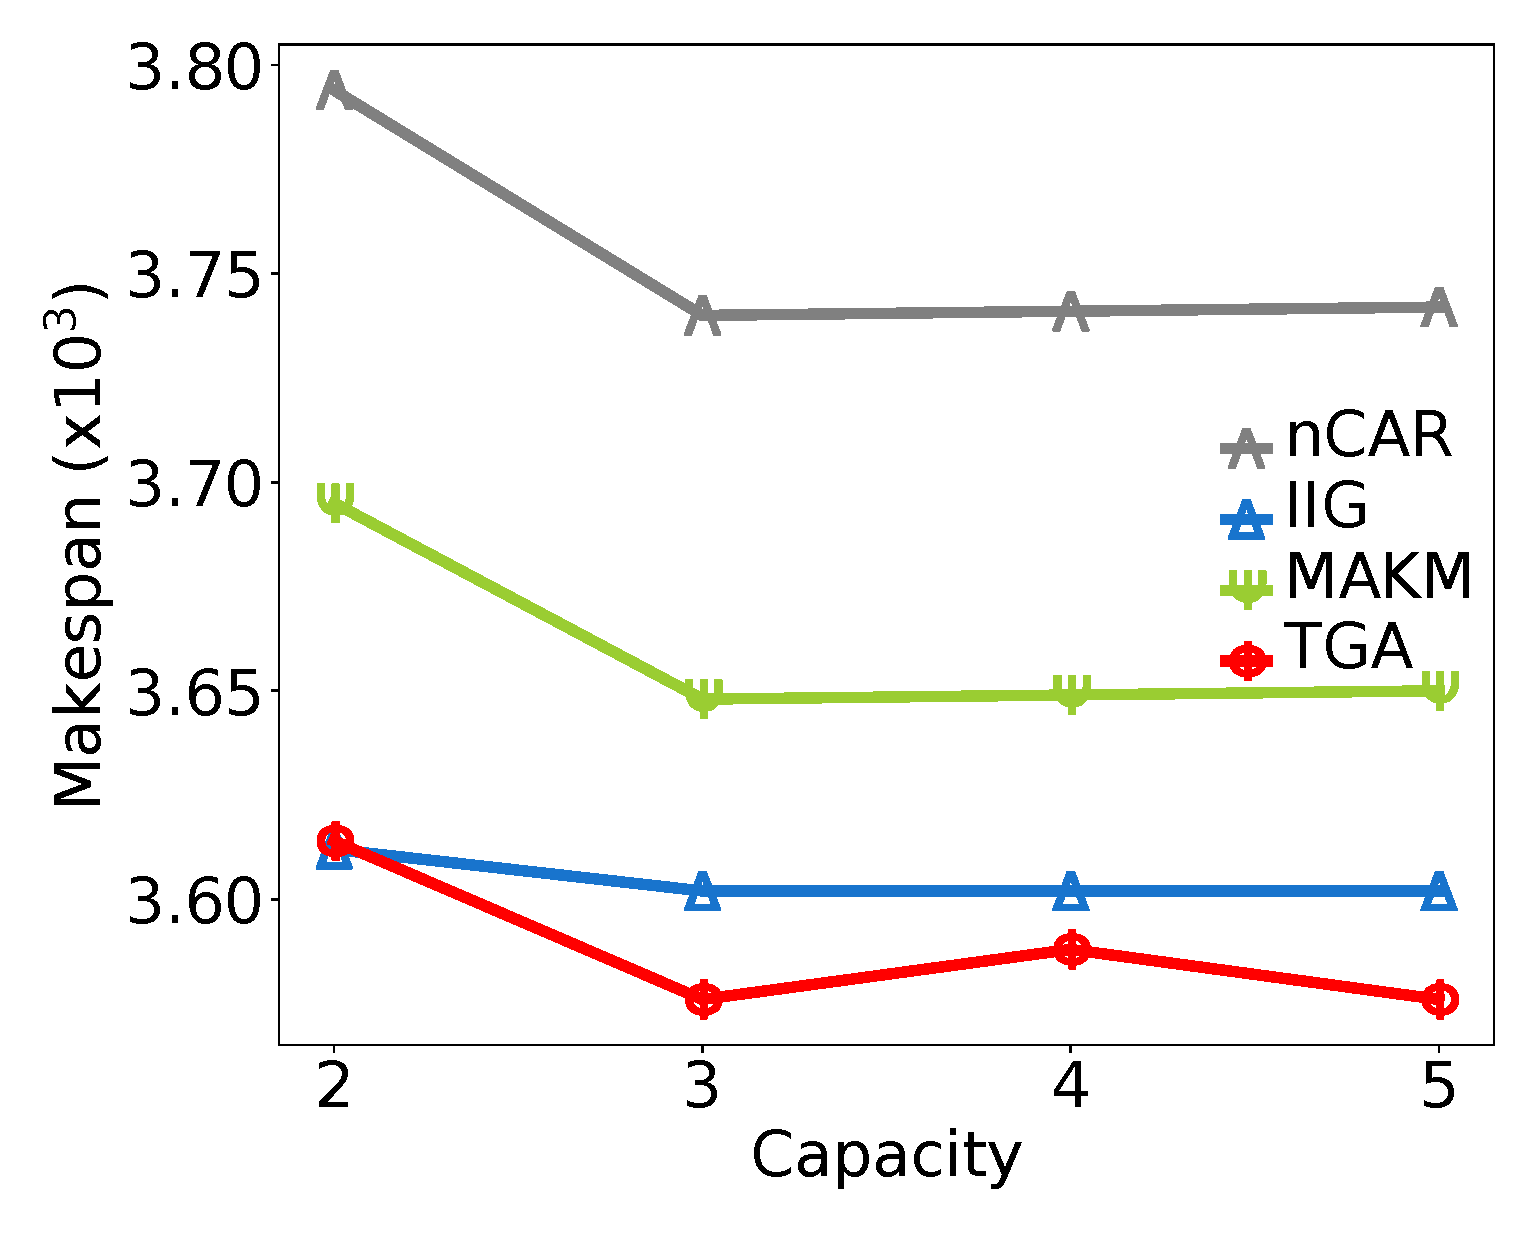
\includegraphics[width=0.3\linewidth]{Fig/capacityMS.eps}}
%   \subfigure[$c$ vs. PT]{
%     \label{fig:ep:capacityPT}
%     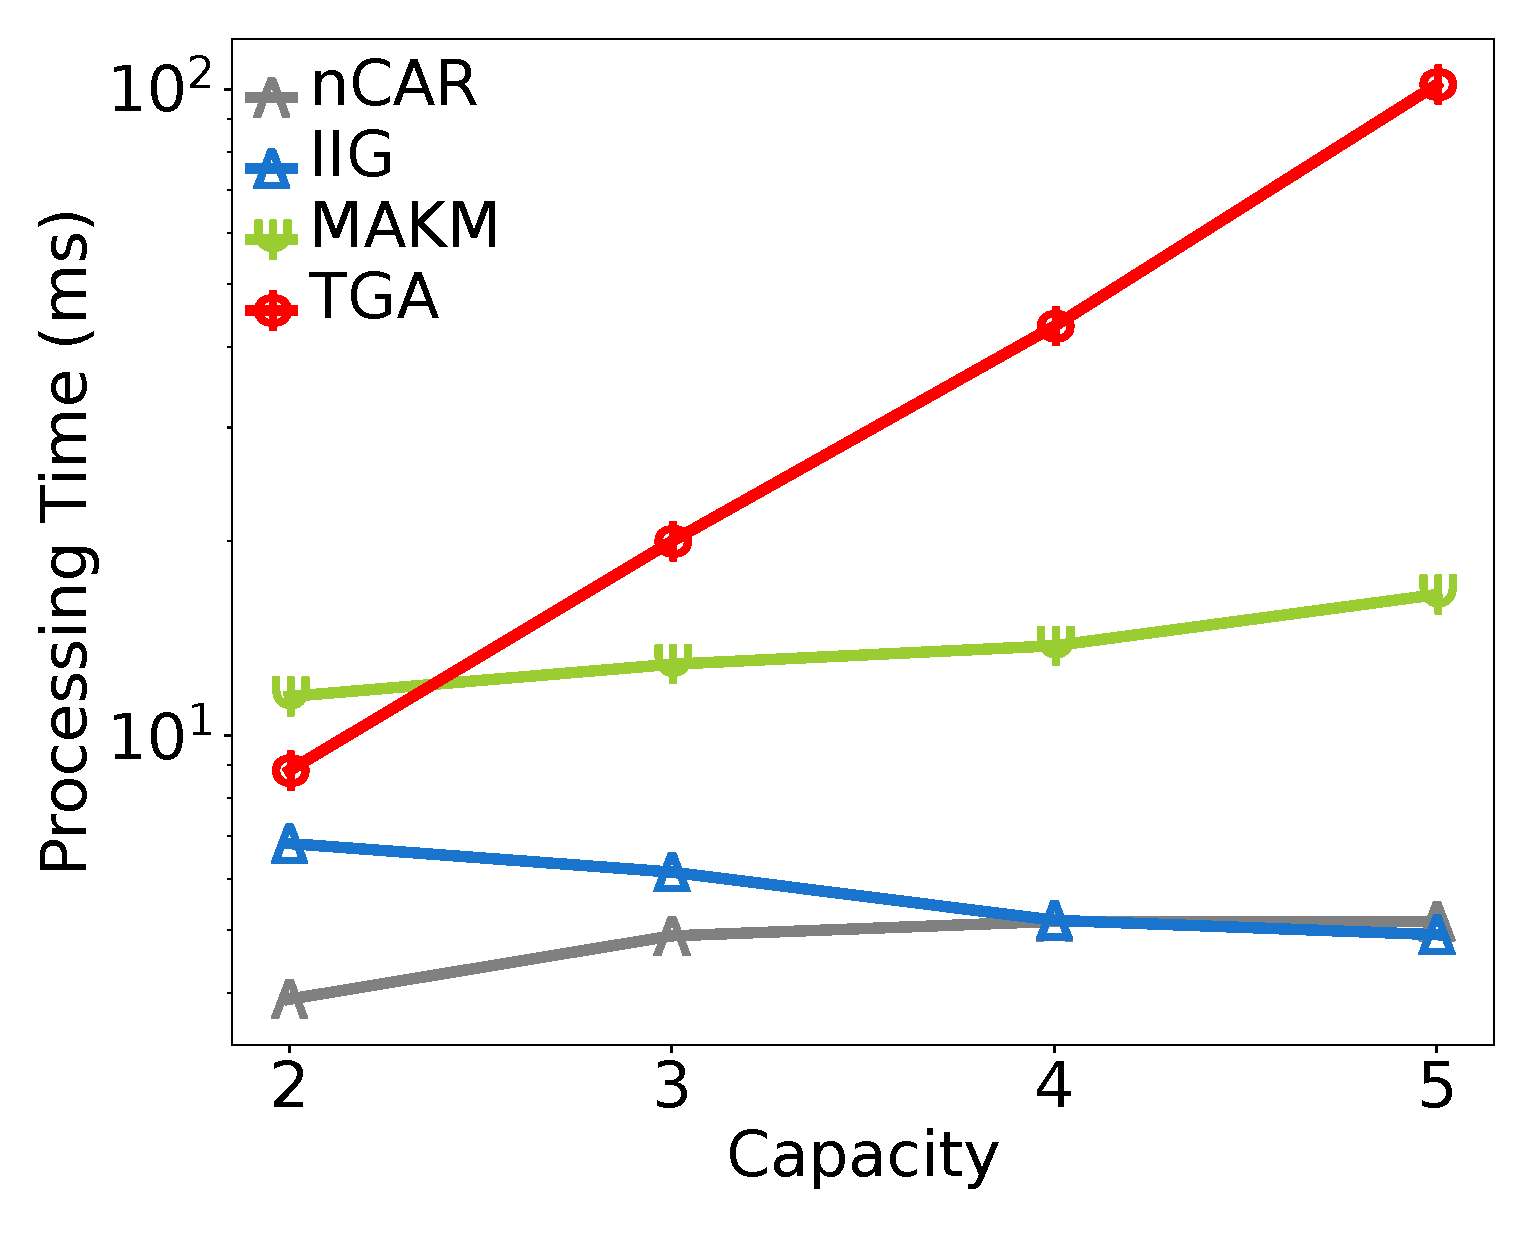
\includegraphics[width=0.3\linewidth]{Fig/capacityPT.eps}}
%   \caption{Performance of $c$ \textbf{vs. ST, MS and PT}}
%   \label{fig:ep:capacity}
%   \Description{Performance of $c$ \textbf{vs. ST, MS and PT}}
% \end{figure*}

\section{Conclusion}
\label{sec:conclusion}
% In this paper, we focus on the carpooling scores between multiple tasks,
% which is a key factor in MLAPD problem.
% We first propose the K-Capacity Hierarchical Clustering Algorithm 
% to divide the set of tasks into groups,
% in which tasks have less impact on each other's completion time.
% Then, we introduce the Task Group Allocation Algorithm to allocate task groups to agents.
% Finally, we conduct experiments to evaluate the performance of the proposed algorithm.

In this paper, we propose the Task Group Allocation Algorithm to solve the MLAPD problem.
We first evaluate the upper bound on the cost of the schedule of multiple tasks,
and quantify the carpooling scores between multiple tasks.
Next, we propose the K-Capacity Hierarchical Clustering Algorithm to divide the set of tasks into groups,
in which tasks have less impact on each other's completion time.
Then, we introduce the Task Group Allocation Algorithm to allocate task groups to agents.
Finally, we conduct experiments to evaluate the performance of the proposed algorithm.
In the future, we will consider
the heterogeneous agents and the dynamic environment in the MLAPD problem,
which is more practical in real-world applications.

\balance

%%%%%%%%%%%%%%%%%%%%%%%%%%%%%%%%%%%%%%%%%%%%%%%%%%%%%%%%%%%%%%%%%%%%%%%%

%%% The acknowledgments section is defined using the "acks" environment
%%% (rather than an unnumbered section). The use of this environment 
%%% ensures the proper identification of the section in the article 
%%% metadata as well as the consistent spelling of the heading.
 
\begin{acks}
  This work is financially supported by Shenzhen Science and Technology Program 
  under Grant No.GXWD20220817124827001 and No.JCYJ20210324132406016.
\end{acks}

%%%%%%%%%%%%%%%%%%%%%%%%%%%%%%%%%%%%%%%%%%%%%%%%%%%%%%%%%%%%%%%%%%%%%%%%

%%% The next two lines define, first, the bibliography style to be 
%%% applied, and, second, the bibliography file to be used.

\bibliographystyle{ACM-Reference-Format} 
\bibliography{sample}

%%%%%%%%%%%%%%%%%%%%%%%%%%%%%%%%%%%%%%%%%%%%%%%%%%%%%%%%%%%%%%%%%%%%%%%%


\end{document}

%%%%%%%%%%%%%%%%%%%%%%%%%%%%%%%%%%%%%%%%%%%%%%%%%%%%%%%%%%%%%%%%%%%%%%%%

% \begin{algorithm}[ht]
% \caption{K-Capacity Hierarchical Clustering Algorithm}
% \label{alg:KCHC}
% \KwIn{Set of tasks $\Gamma$, the max capacity of agents $K$}
% \KwOut{Set of task groups ${\Pi}$}
% Initialize ${\Pi} = \emptyset$
% \For {$\tau_{i} \in \Gamma$}{
%     Treat $\tau_{i}$ as a task group $\Gamma_{i}$, and add $\Gamma_{i}$ into ${\Pi}$
%     Calculate the carpooling scores between $\tau_{i}$ and other tasks in $\Gamma$
% }
% \Return$\Pi$
% \end{algorithm}